% ************************************************************************
%
% Automated neuron detection in high-content fluorescence microscopy images
% using machine learning 
%
% ************************************************************************
\chpos{15mm}{8mm}
\chapter[Automated neuron detection in high-content fluorescence microscopy images using machine learning]{Automated neuron detection in high-content fluorescence microscopy images using machine learning}
\chaptermark{Automated neuron detection in high-content images using machine learning}
\label{ch5:ndetchml}
% abstract
{\small \lettrine{T}{he} study of neuronal morphology in relation to function, and the development of effective medicines to positively impact this relationship in patients suffering from neurodegenerative diseases, increasingly involves image-based high-content screening and analysis. The first critical step toward fully automated high-content image analyses in such studies is to detect all neuronal cells and distinguish them from possible non-neuronal cells or artifacts in the images. In this chapter, the performance of well-established machine learning techniques is investigated for this purpose. These include support vector machines, random forests, k-nearest neighbors, and generalized linear model classifiers, operating on an extensive set of image features extracted using the compound hierarchy of algorithms representing morphology, and the scale-invariant feature transform. The experiments performed on a dataset of rat hippocampal neurons are presented in order to find the most suitable classifier(s) and subset(s) of features in the common practical setting where there is very limited annotated data for training. The results indicate that a random forests classifier using the right feature subset ranks best for the considered task, although its performance is not statistically significantly better than some support vector machine based classification models.\par}
\vspace*{12em}
% ************************************************************************
\begin{publish}
	Based upon: G. Mata, M. Radojevi\'{c}, C. Fernandez-Lozano, I. Smal, N. Werij, M. Morales, E. Meijering, J. Rubio, ``Automated neuron detection in high-content fluorescence microscopy images using machine learning'', \textit{Neuroinformatics}, \textit{in press}, 2018.%vol. 0, no. 0, pp.0-0
\end{publish}

\section{Introduction}
\label{ch5:sec:intro}

Neurons are special cells in the sense that they codify and transmit information in the form of action potentials. Networks consisting of many billions of neurons, such as in the brains of higher organisms, are extraordinarily complex and perform many different functions. Since the pioneering work of \cite{ramon2008histologia} it is well known that the morphology of neurons vary widely in different parts of the brain and that neuronal morphology and function are intricately linked. Moreover, in healthy conditions, neuronal (sub)networks within the brain are dynamic and continuously readjust their connections during the lifetime of an organism in response to external stimuli, in order to refine existing functions or learn new ones \cite{ascoli2015trees}. Conversely, in pathological conditions, disease processes destructively alter neuronal morphology and cause progressive loss of function, such as in Alzheimer's and Parkinson's disease, but also in aging \cite{van2001need}. Thus the study of neuronal cell morphology in relation to function, in health and disease, is of high importance for developing suitable drugs and therapies \cite{meijering2010neuron}.

A convenient tool to visualize large numbers of cultured cells for phenotypic profiling and analysis in drug discovery is high-content fluorescence microscopy imaging \cite{xia2012concise, antony2013light, singh2014increasing, bougen2017large}. By automated acquisition it produces very large amounts of image data, which cannot be analyzed manually but require automated high-content analysis (\gls{hca}) in order to take full advantage of all captured information. \gls{hca} is also used increasingly in neuroscience research \cite{dragunow2008high, anderl2009neuronal, jain2012high} and various image processing pipelines have been developed for quantitative analysis of neuronal cells in high-content images \cite{vallotton2007automated, zhang2007novel, wu2010automatic, dehmelt2011neuritequant, radio2012neurite, charoenkwan2013hcs, smafield2015automatic}. However, especially in screening applications, where the image quality is often relatively low and may vary widely between experiments, the challenge remains to develop more accurate and more robust image analysis methods \cite{sommer2013machine, kraus2016computer, meijering2016imagining}.

The first critical step in any HCA pipeline is the detection of the objects of interest in the images. It is well recognized now in many areas of microscopic image analysis that machine learning based classification methods are an excellent choice for this task and typically outperform non-learning methods based on manually defined rules \cite{horvath2011machine, sommer2013machine, kraus2016computer, arganda2017trainable}. However, which classifiers work best, and on which sets of image features, may depend on the specific image data and detection task, and needs to be determined experimentally before using HCA on a routine basis in a given application.

This chapter comprises the investigation of the performance of machine learning methods for the specific task of detecting neuronal cells in high-content fluorescence microscopy images as a first step toward fully automated HCA in conduced neuroscientific studies. An early version of this work was presented at a conference \cite{mata2016automatic} while the chapter reports on a significant extension of that work including more classifiers, more extensive experiments and results, and a much deeper and more solid (statistical) analysis and discussion of the findings. The classifiers are explored based on precalculated image features in order to determine which combinations of classifiers and features work best in a practical setting where there is very limited annotated data for training. Specifically, various state-of-the-art classifiers are considered based on support vector machines (\gls{svm}), random forests (\gls{rf}), k-nearest neighbors (KNN), and generalized linear models (in particular GLMNET), operating on more than a thousand image features extracted using the compound hierarchy of algorithms representing morphology (CHARM) and the scale-invariant feature transform (\gls{sift}).
\begin{figure}%[ht]
	\centering
	\begin{subfigure}{\textwidth}
		\centering
		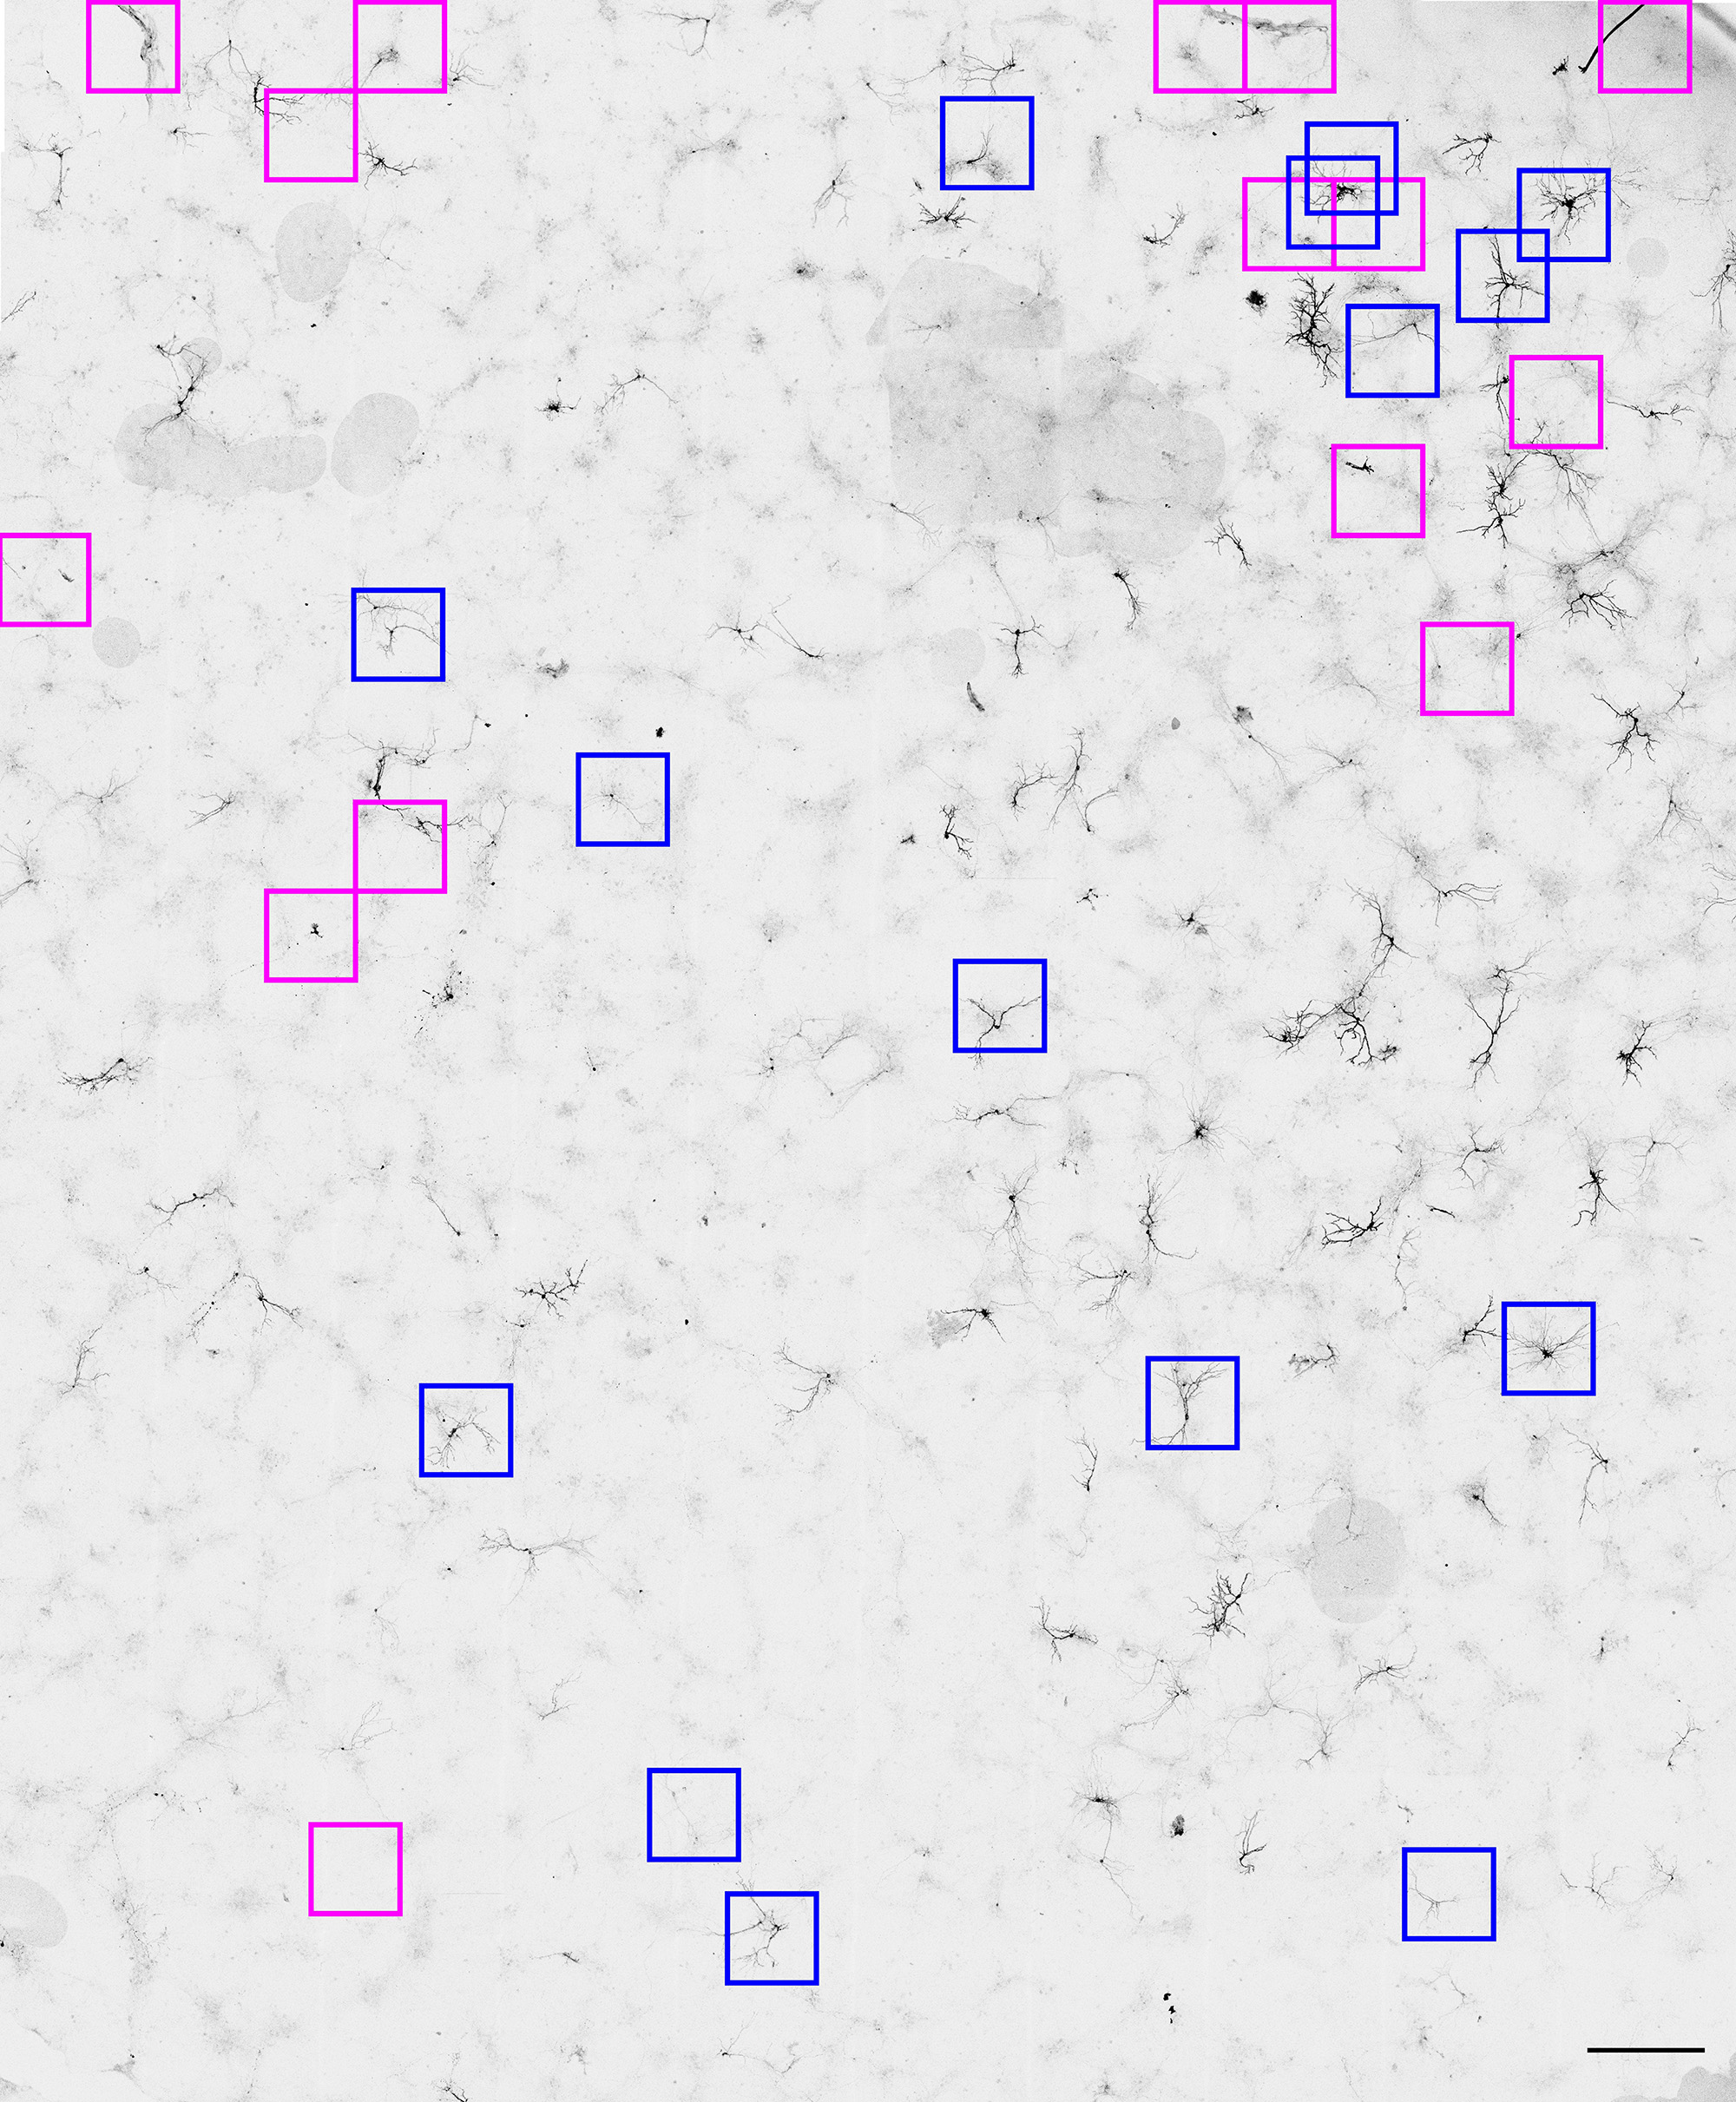
\includegraphics[width=0.7\textwidth]{fig01a}
		\vspace{-0.5em}
		\caption{Example high-content image. Scale bar: 500$\mu$m.}
		\vspace{1em}
	\end{subfigure}
	\begin{subfigure}{0.45\textwidth}
		\centering
		\begin{tabular}{c@{\,}c@{\,}c@{\,}c@{\,}c@{}}
			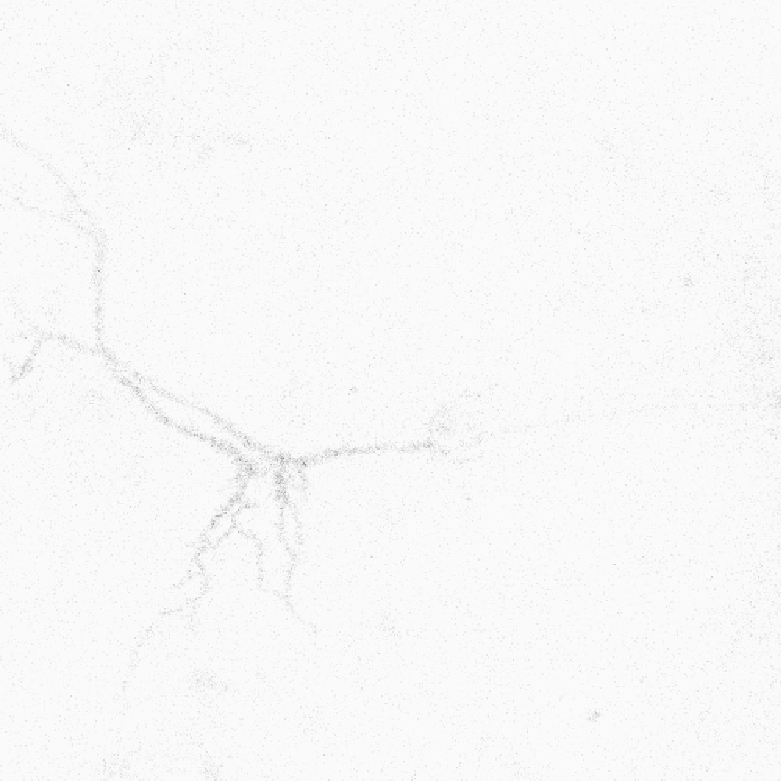
\includegraphics[width=0.19\textwidth]{fig01b01} &
			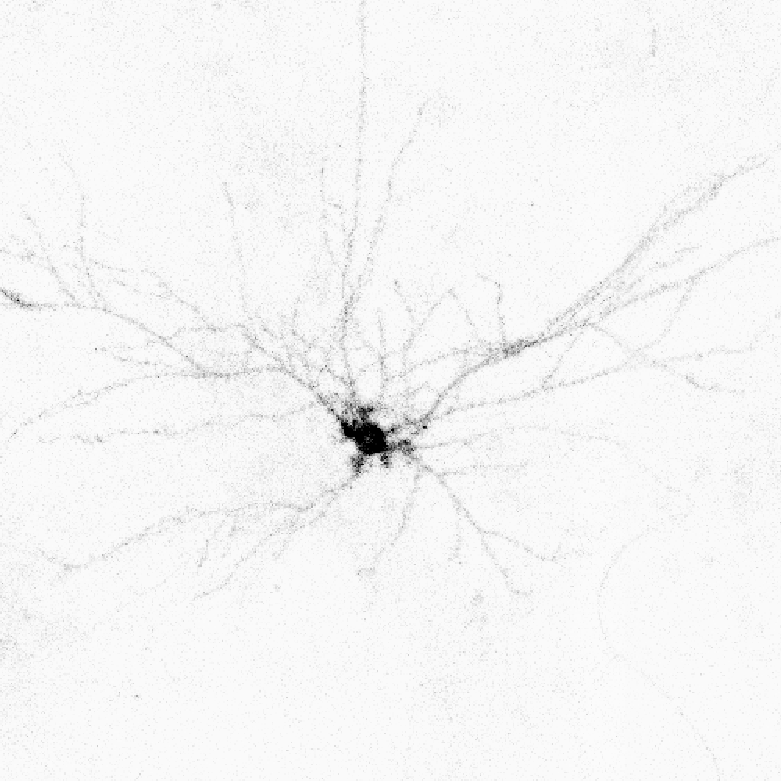
\includegraphics[width=0.19\textwidth]{fig01b02} &
			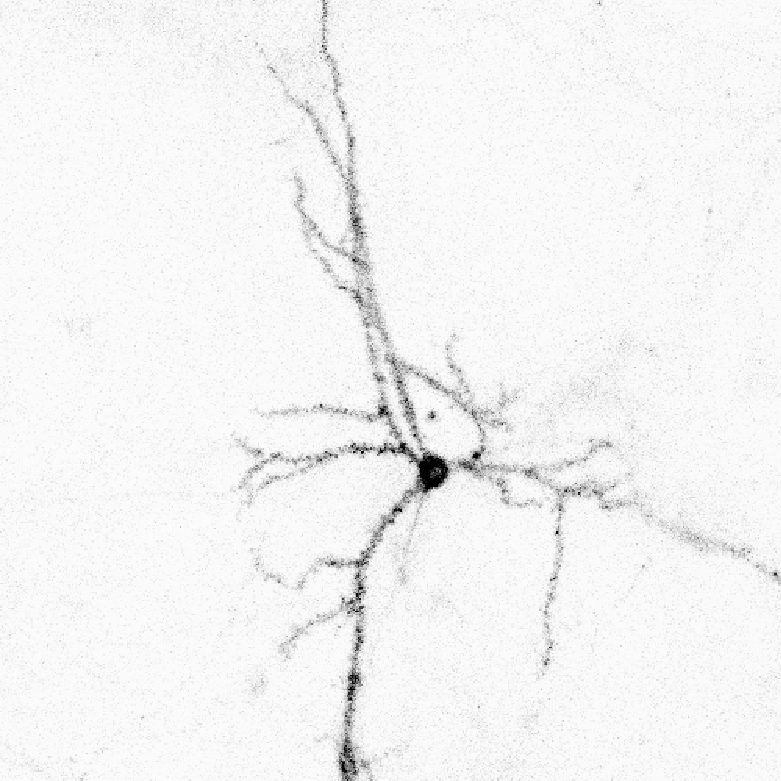
\includegraphics[width=0.19\textwidth]{fig01b03} &
			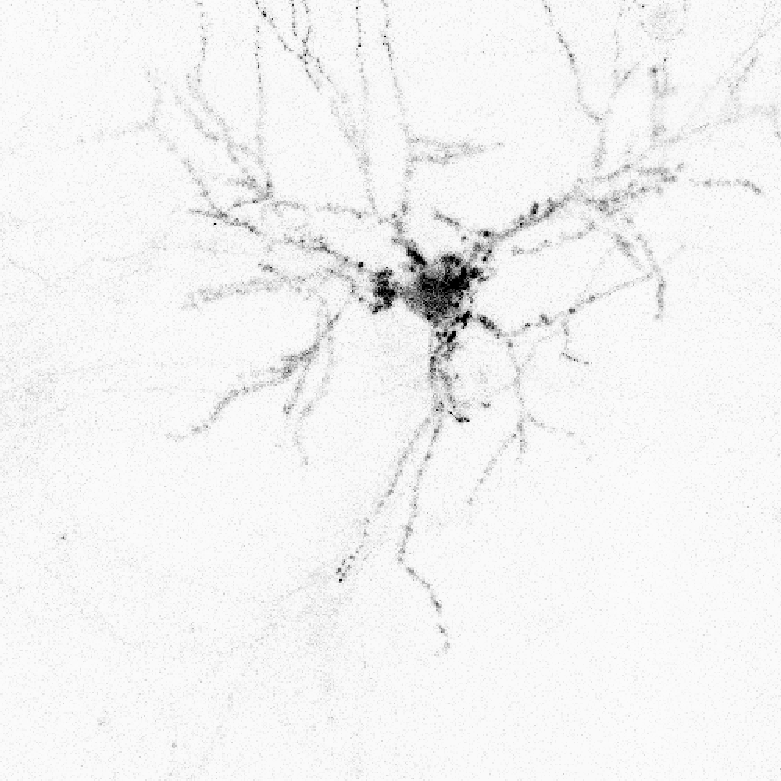
\includegraphics[width=0.19\textwidth]{fig01b04} &
			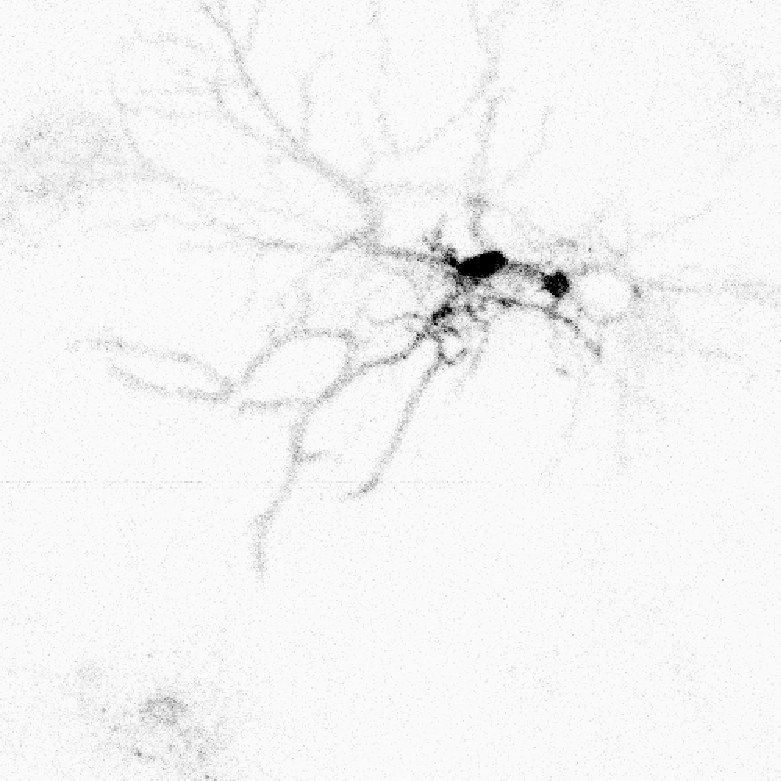
\includegraphics[width=0.19\textwidth]{fig01b05} \\
			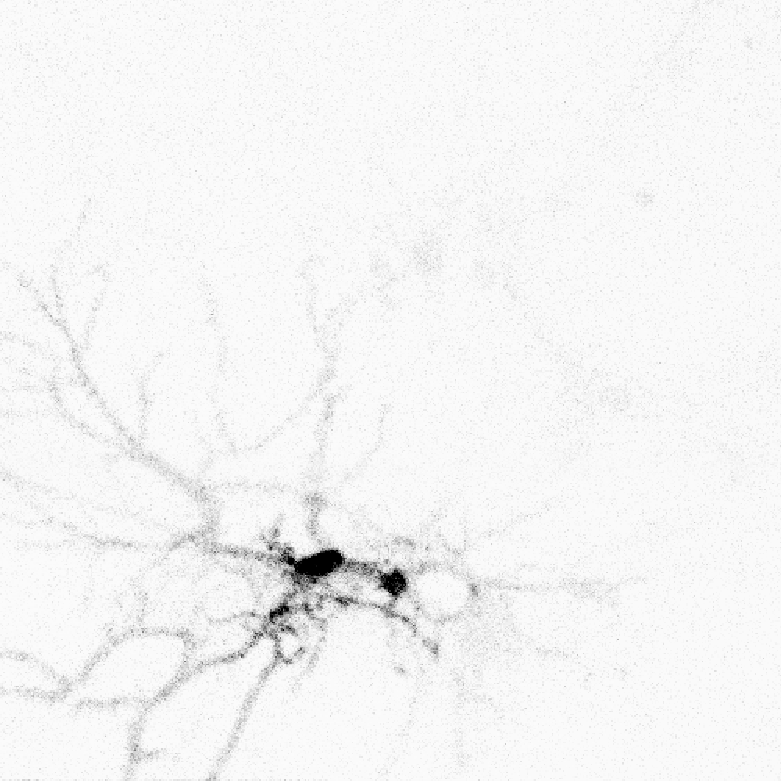
\includegraphics[width=0.19\textwidth]{fig01b06} &
			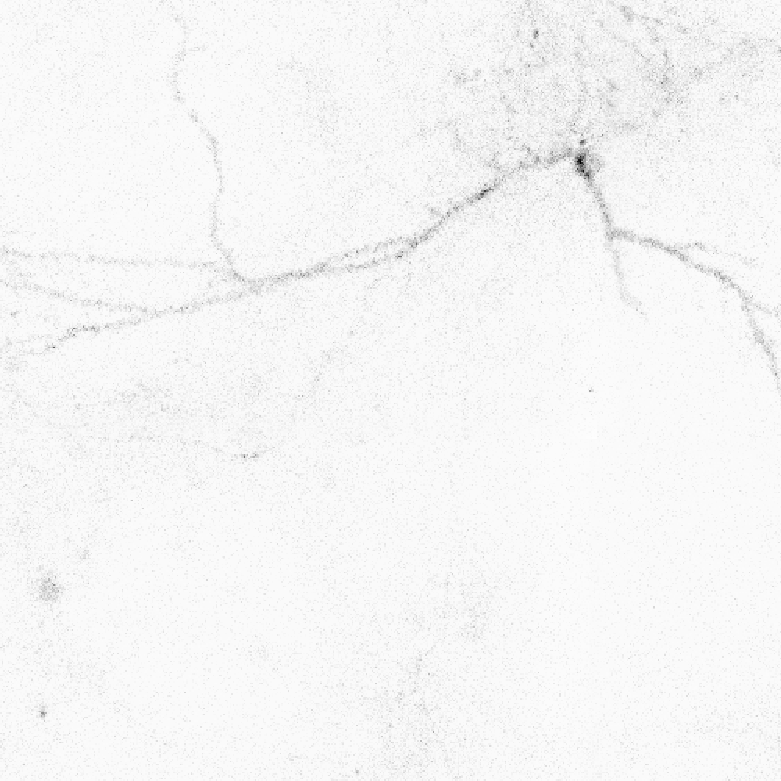
\includegraphics[width=0.19\textwidth]{fig01b07} &
			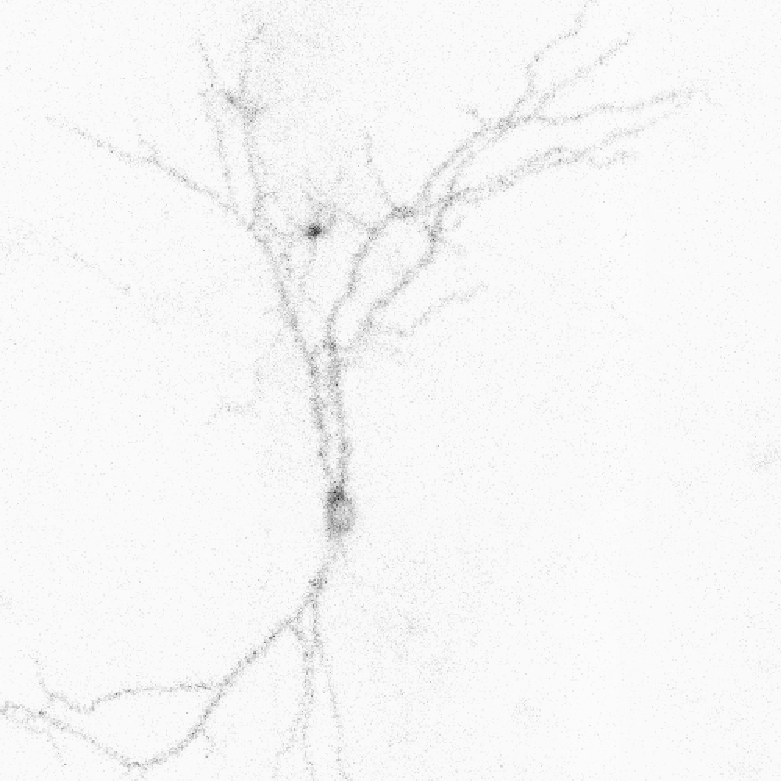
\includegraphics[width=0.19\textwidth]{fig01b08} &
			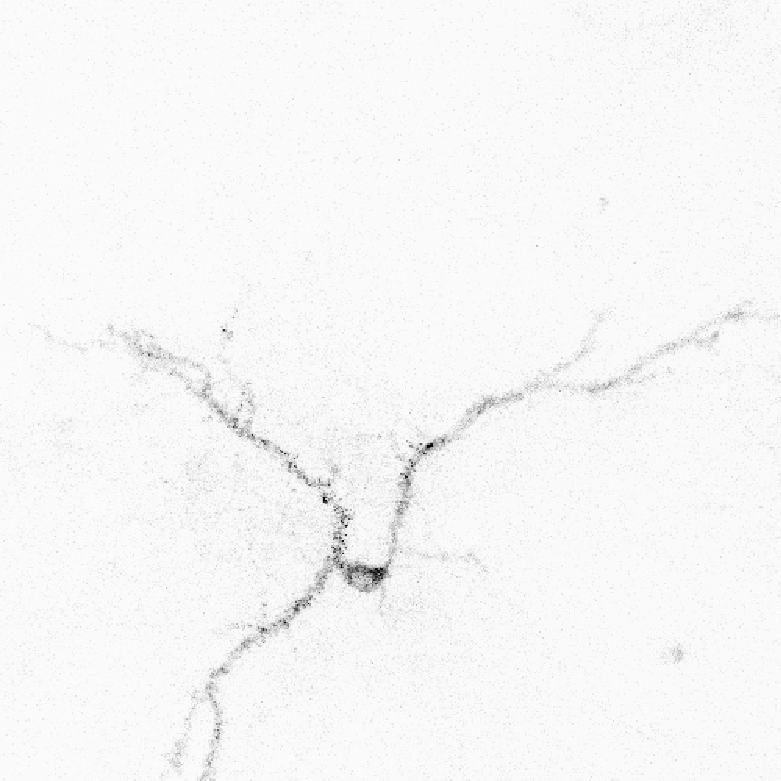
\includegraphics[width=0.19\textwidth]{fig01b09} &
			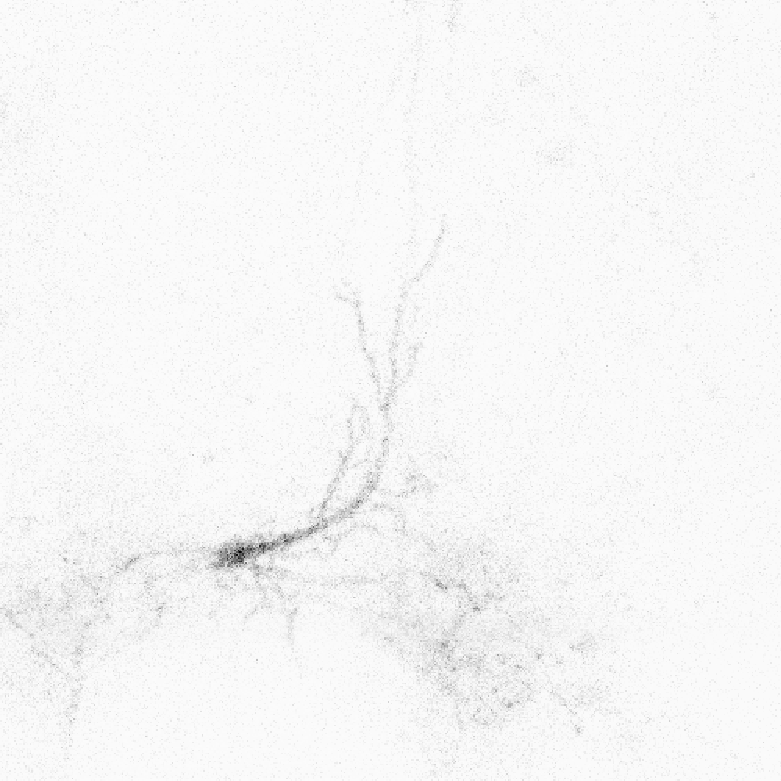
\includegraphics[width=0.19\textwidth]{fig01b10} \\
			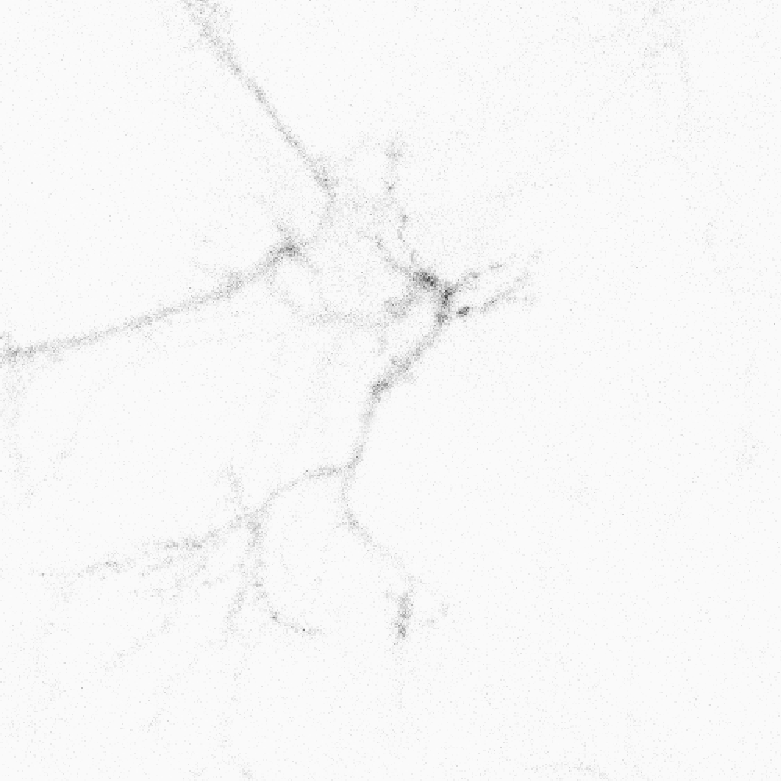
\includegraphics[width=0.19\textwidth]{fig01b11} &
			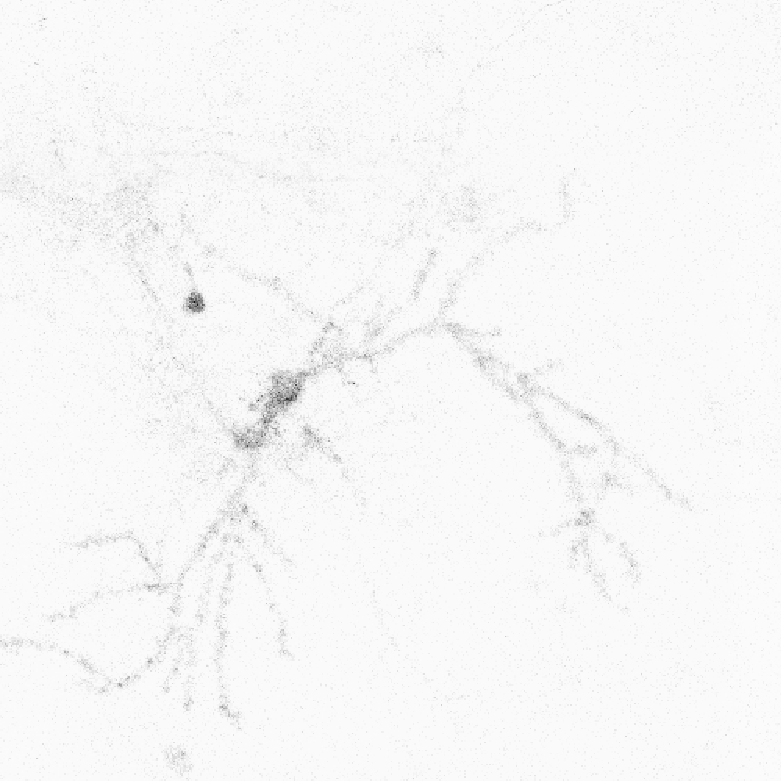
\includegraphics[width=0.19\textwidth]{fig01b12} &
			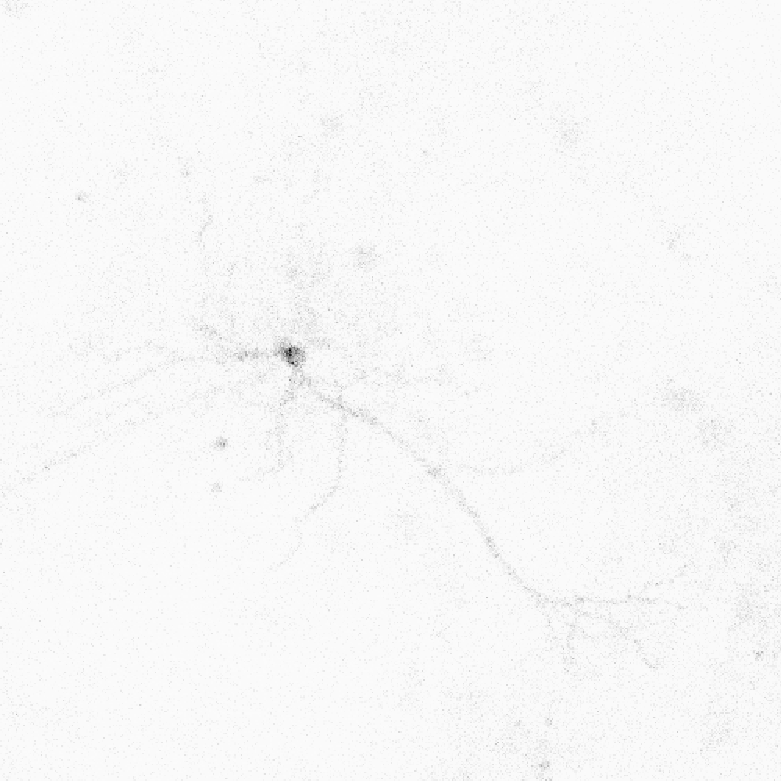
\includegraphics[width=0.19\textwidth]{fig01b13} &
			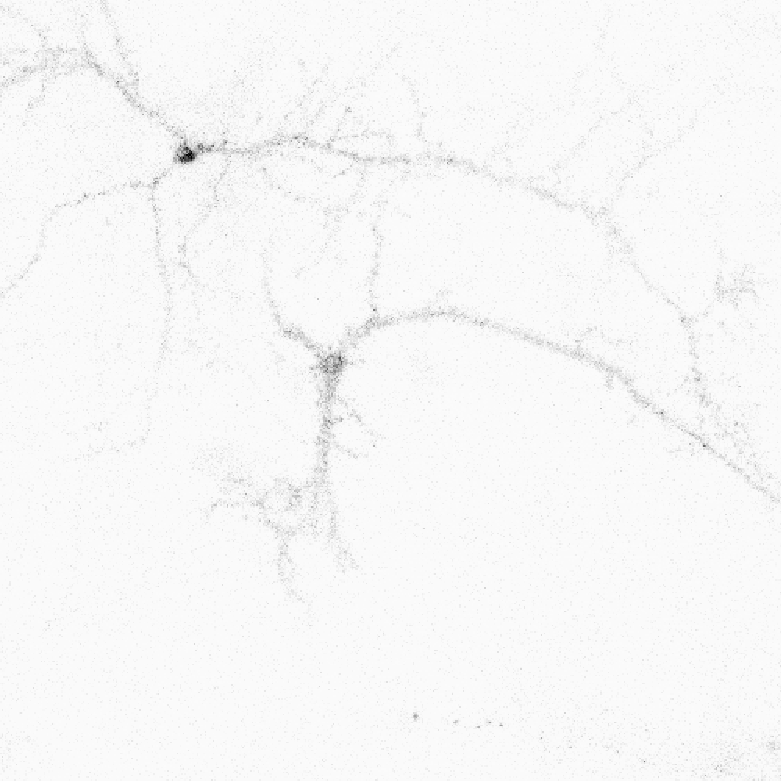
\includegraphics[width=0.19\textwidth]{fig01b14} &
			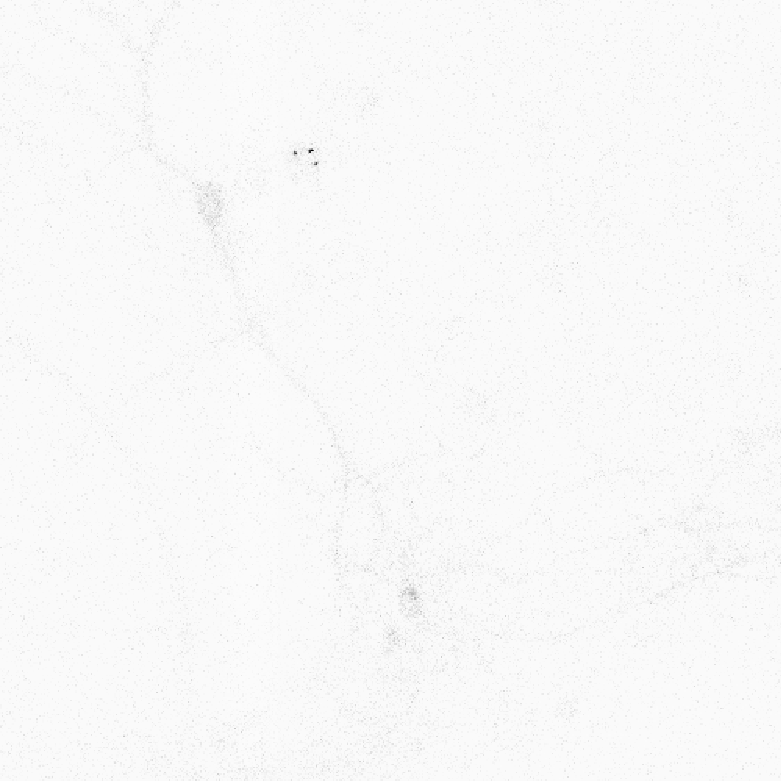
\includegraphics[width=0.19\textwidth]{fig01b15}
		\end{tabular}
		\vspace{-0.5em}
		\caption{Example patches considered as positives (blue squares).}
%		\vspace{1em}
	\end{subfigure}
	\hspace{0.05\textwidth}
	\begin{subfigure}{0.45\textwidth}
		\centering
		\begin{tabular}{c@{\,}c@{\,}c@{\,}c@{\,}c@{}}
			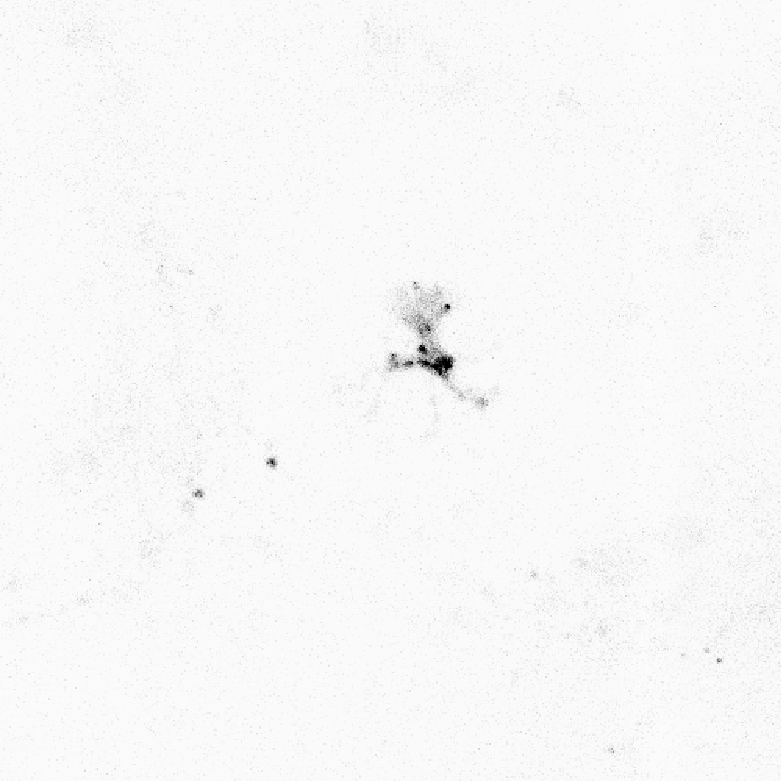
\includegraphics[width=0.19\textwidth]{fig01c01} &
			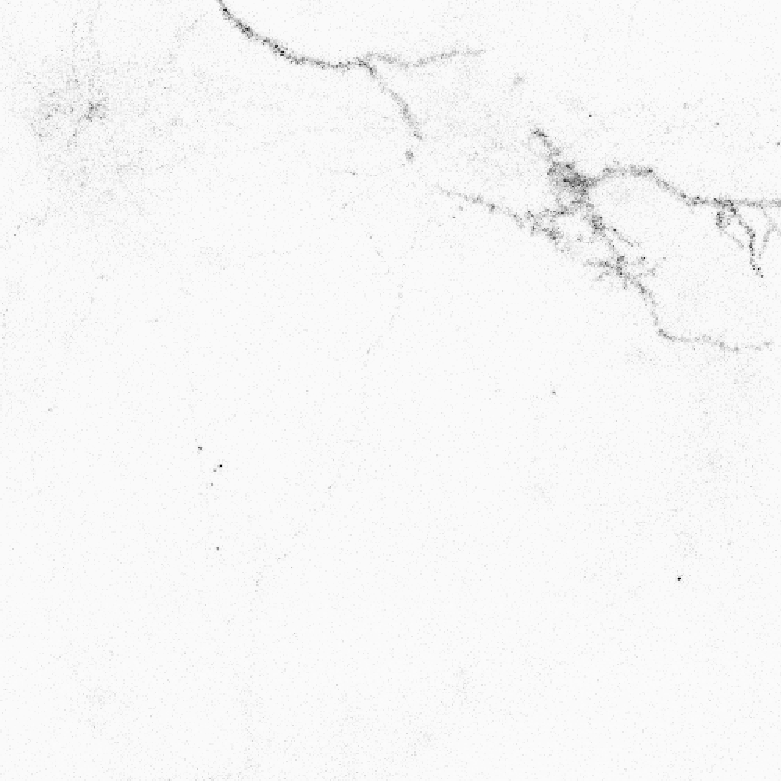
\includegraphics[width=0.19\textwidth]{fig01c02} &
			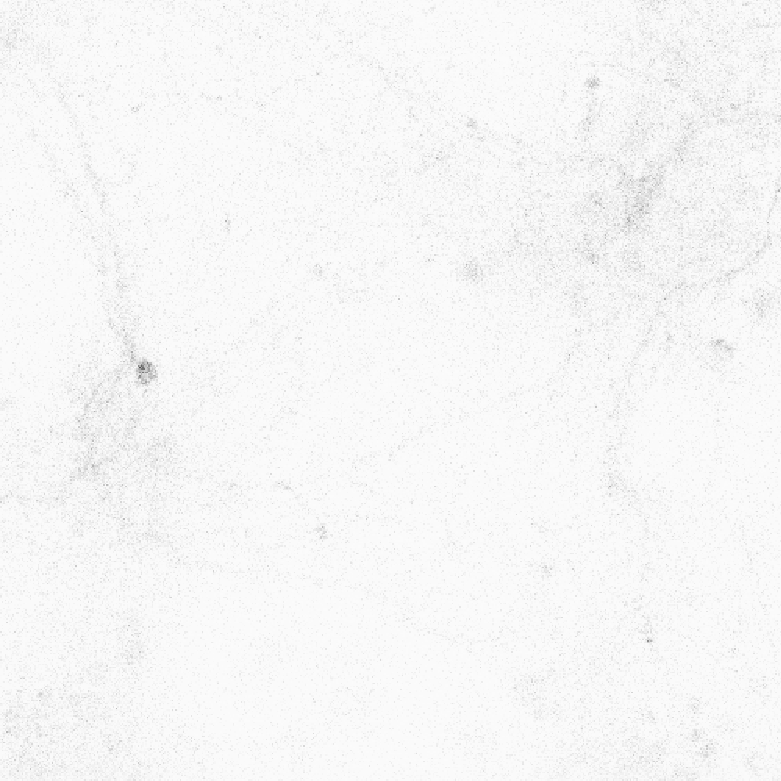
\includegraphics[width=0.19\textwidth]{fig01c03} &
			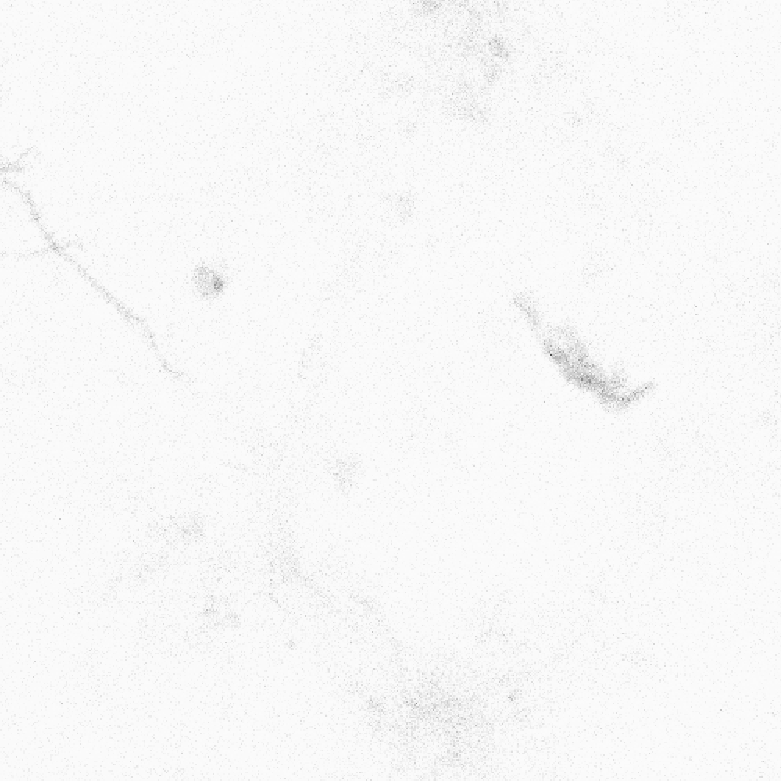
\includegraphics[width=0.19\textwidth]{fig01c04} &
			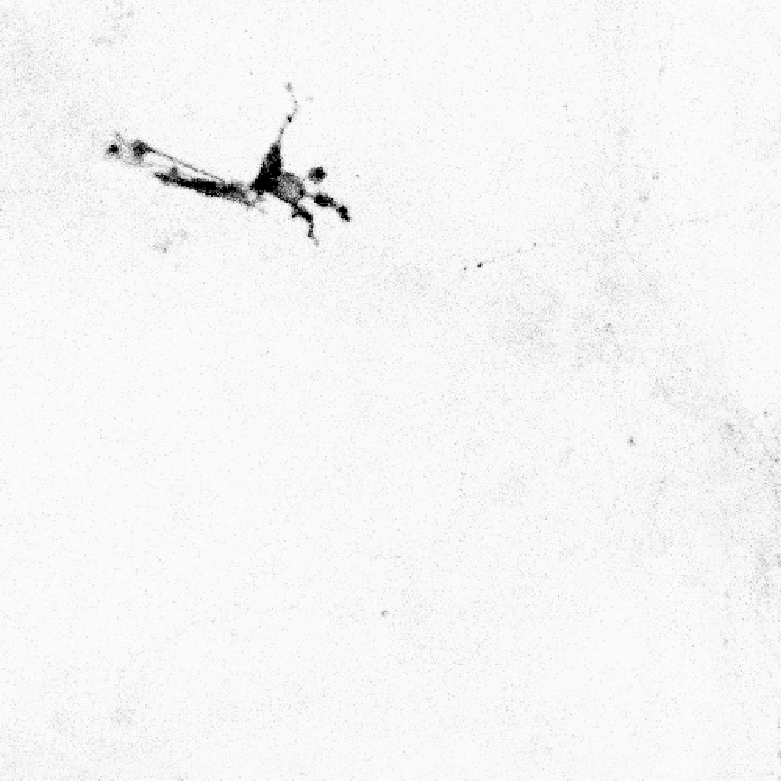
\includegraphics[width=0.19\textwidth]{fig01c05} \\
			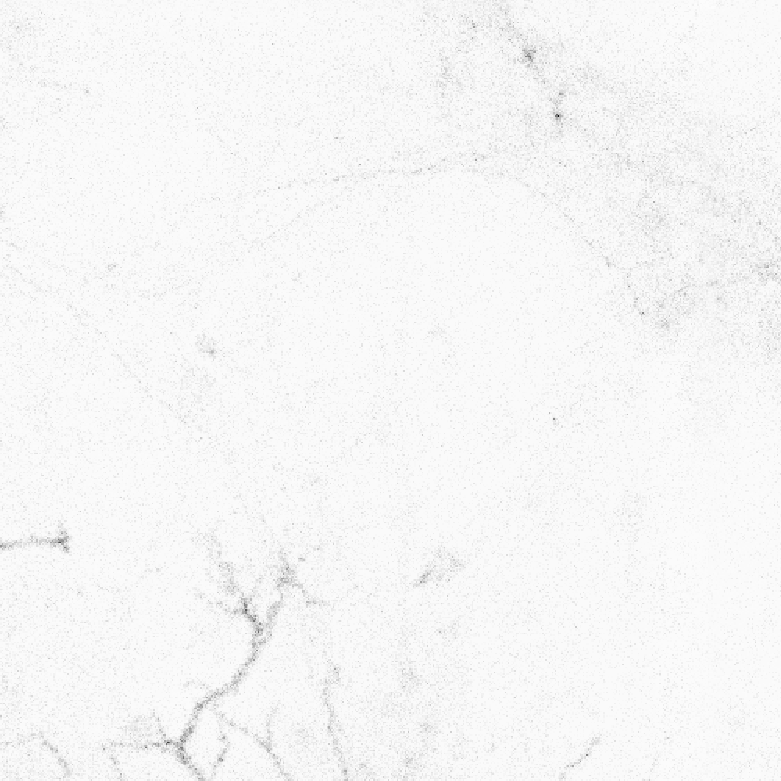
\includegraphics[width=0.19\textwidth]{fig01c06} &
			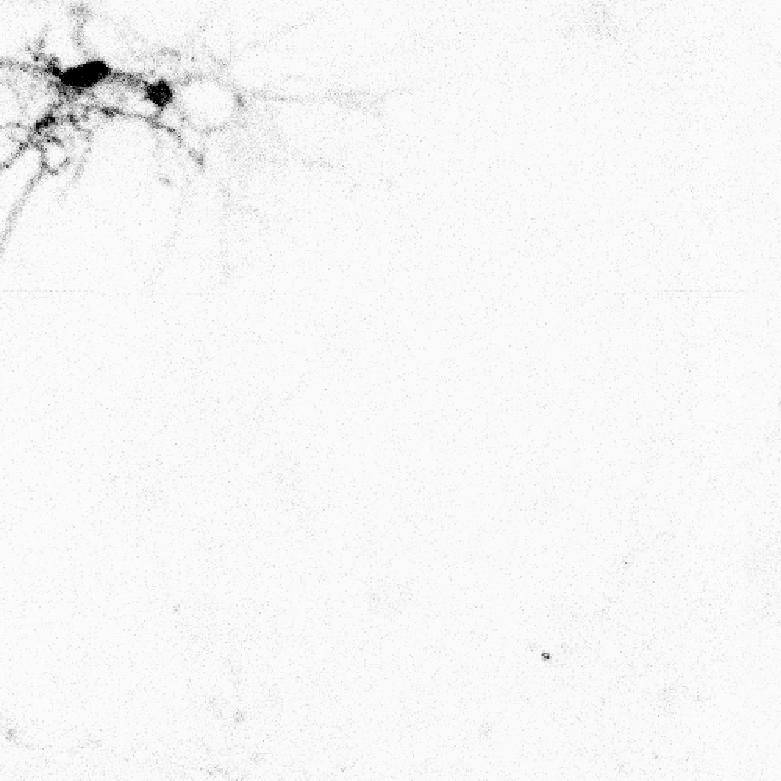
\includegraphics[width=0.19\textwidth]{fig01c07} &
			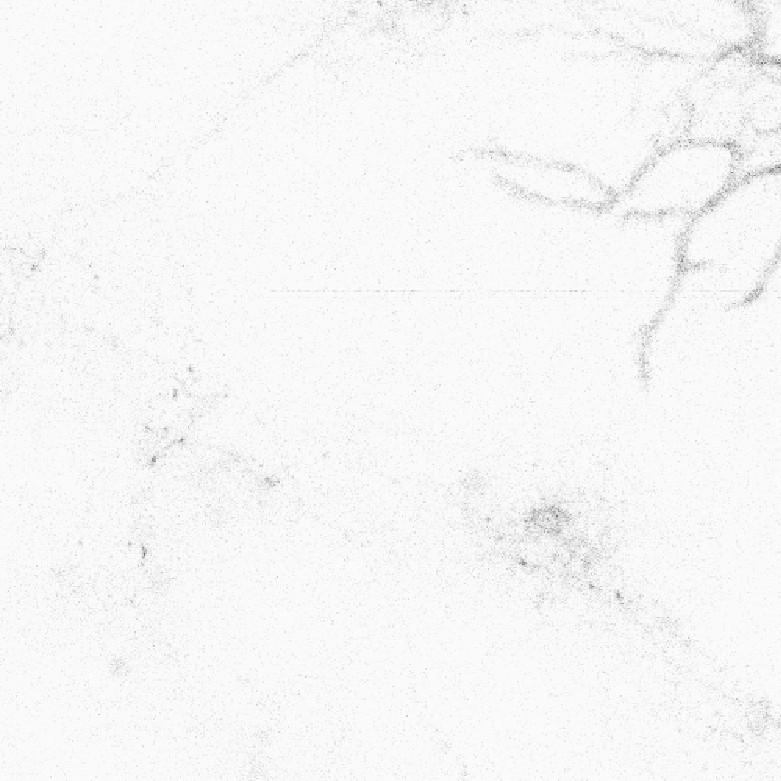
\includegraphics[width=0.19\textwidth]{fig01c08} &
			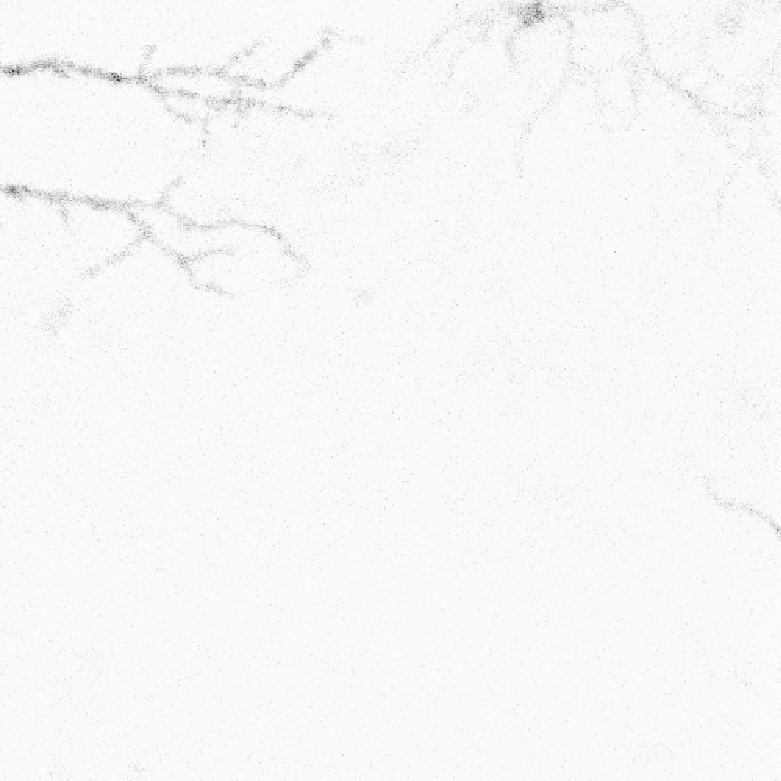
\includegraphics[width=0.19\textwidth]{fig01c09} &
			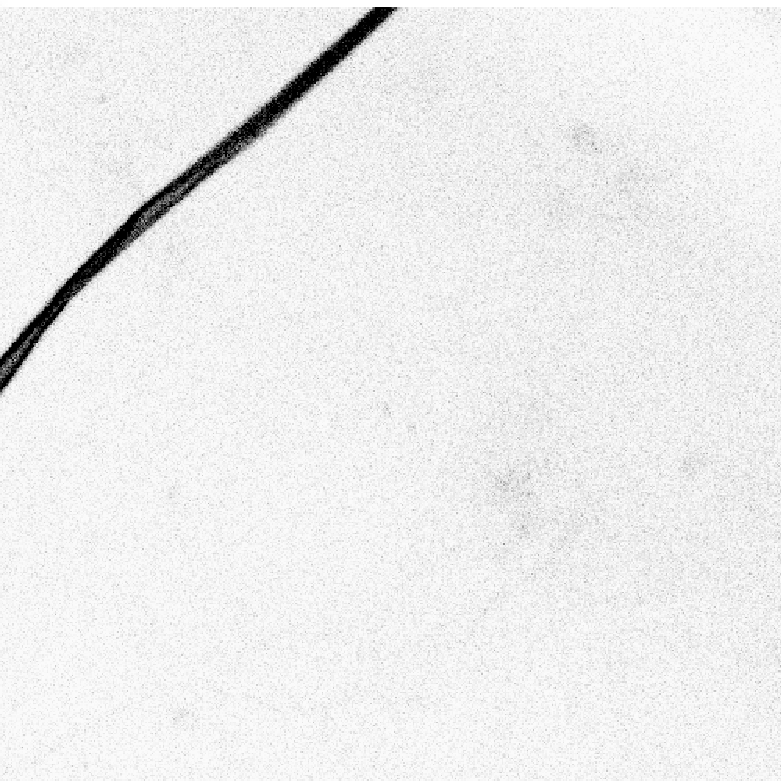
\includegraphics[width=0.19\textwidth]{fig01c10} \\
			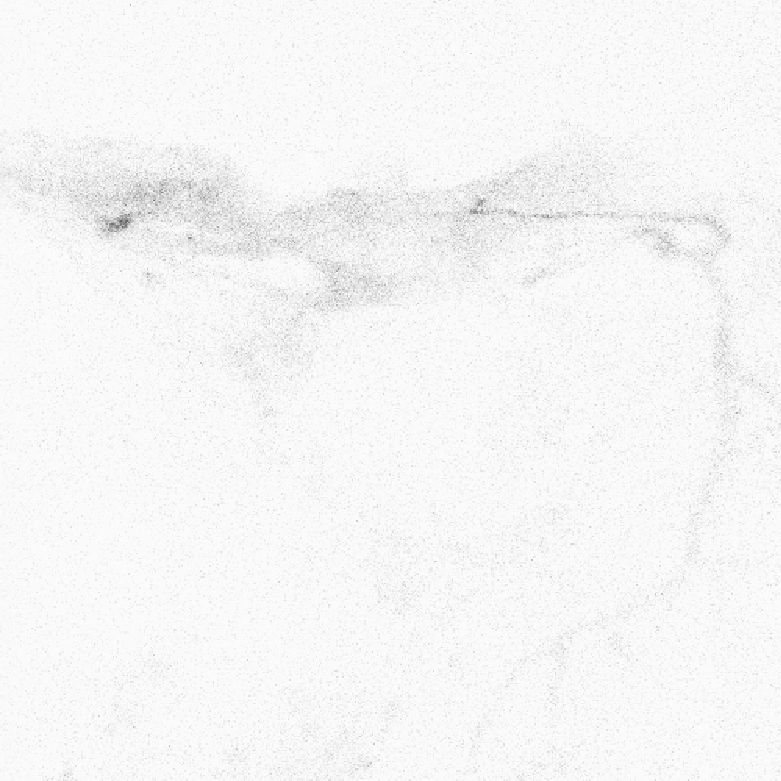
\includegraphics[width=0.19\textwidth]{fig01c11} &
			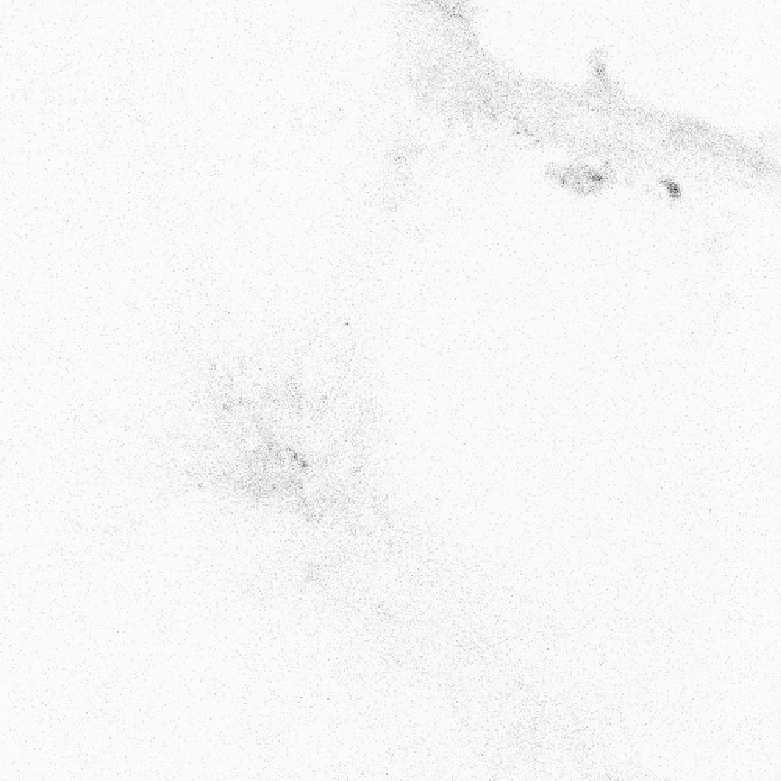
\includegraphics[width=0.19\textwidth]{fig01c12} &
			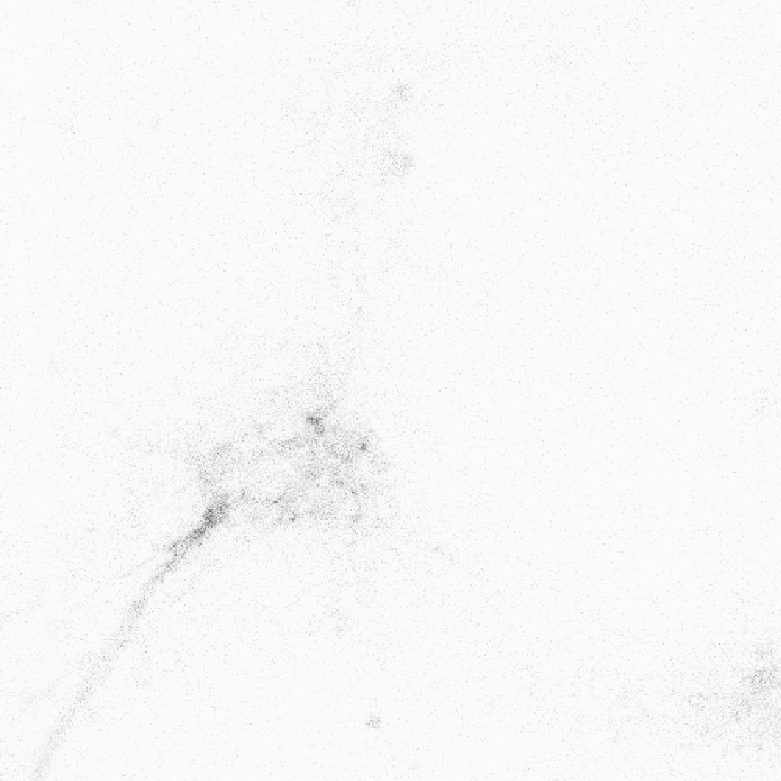
\includegraphics[width=0.19\textwidth]{fig01c13} &
			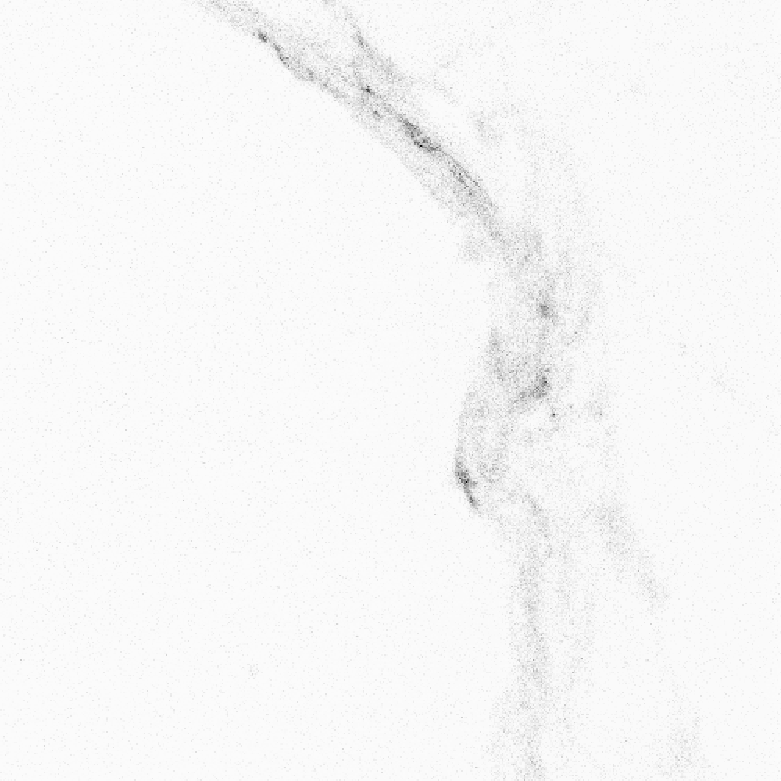
\includegraphics[width=0.19\textwidth]{fig01c14} &
			
\includegraphics[width=0.19\textwidth]{fig01c15}
		\end{tabular}
		\vspace{-0.5em}
		\caption{Example patches considered as negatives (magenta squares).}
	\end{subfigure}	
	\caption{Part of a high-content fluorescence microscopy image (a) where the blue squares highlight some example patches containing neuronal structure and the magenta squares depict some example patches containing background. These squares are enlarged in (b) and (c) for a better visualization. The intensities of the shown images are inverted compared to their originals for displaying purposes.}
	\label{ch5_fig1}
\end{figure}
\section{Materials and methods}
\label{sec:matmet}
The published image data were used and publicly available software tools were employed to facilitate the reproducibility of presented study. This section successively describes the image dataset, the used methods for extracting image features, and the considered machine learning methods\footnote{Materials and methods are available from \url{www. unirioja.es/cu/jurubio/ANDHCFMIUML}}.

\subsection{Image dataset}
\label{sec:data}

The high-content image data used in this study originates from the ongoing research aimed at discovering effective treatments for neurological disorders \cite{cuesto2011phosphoinositide, enriquez2014learning, enriquez2016pi3k}. The acquisition of the images is described, their annotation, and the strategy used to obtain a well-balanced dataset for training of the machine learning algorithms.

\subsubsection{Image acquisition}
\label{sec:acquisition}
Rat hippocampal neurons were cultured and transfected with green fluorescent protein (\gls{gfp}) and imaged with a Leica SP5 automated confocal fluorescence microscope using its Matrix modules and a 20$\times$ lens. The imaged neurons, coming from a part of the brain (the hippocampus) that is well known to be involved in higher functions such as learning and memory \cite{squire1992memory}, typically have a pyramidal soma with a complex dendritric tree \cite{goslin1998rat}, and their in-vivo morphological features are well conserved in culture conditions. Eight two-dimensional (2D) high-content images were acquired (total size $>$1 GB), each with a size of about 10,000\,$\times$\,12,000 pixels, covering approximately 70\,mm${}^2$ of culture dish. Each image is a mosaic made up of tiles of size 1024\,$\times$\,1024 pixels, automatically acquired and stitched using the Leica Matrix module. Prior to imaging, the user has to select the desired culture area within the field of view, and the module calculates the tiles to be imaged in order to cover the chosen area, considering 10\% overlap between neighboring tiles. Each mosaic contains on the order of 40 transfected neurons (Fig.\ \ref{ch5_fig1}). The used specimens usually have about 100 neurons, but more than half of them are not or only partly imaged, as they are in different optical planes or close to the borders of the dish, making the automated detection of relevant image structures (complete neurons) as opposed to irrelevant image structures (incomplete neurons, astrocytes, and artifacts) quite challenging.

\subsubsection{Image annotation}
\label{sec:annotation}
To obtain a reference dataset for training and testing of the machine learning methods, an expert neurobiologist manually marked all the regions of interest (ROIs) containing neurons in these images, about 400 in total. It was established upon data inspection that relevant neurons typically cover an area of around 500 $\times$ 500 pixels in the used images and therefore the ROI size was fixed to these dimensions. Using the same window size, additional patches were automatically sampled from the remaining parts of the images, containing all different types of irrelevant image structures. More specifically, to ensure evenly distributed sampling of background patches across the images, a regular grid is defined, including every patch from the grid having less than 50\% overlap with any of the neuron ROIs marked by the expert, resulting in approximately 4,500 non-neuron patches. In the sequel, neuron ROIs are referred to as `positives' and the non-neuron image patches as `negatives' (Fig.~\ref{ch5_fig1}).

\subsubsection{Dataset balancing}
\label{sec:balanced}
Due to the neuron sparseness within the image data, the patches of the negative class far outnumbered those of the positive class, with a ratio of approximately 10:1, resulting in an imbalanced dataset. It is well known that the performance of classification algorithms may be negatively impacted by the data being imbalanced \cite{chawla2004editorial, daskalaki2006evaluation, forman2010apples, branco2016survey}, as the algorithms may overfit the majority class and underfit the minority class, and favor the former, yielding biased results \cite{garcia2014bias, li2018adaptive}. Approaches to deal with class imbalance can roughly be divided into two categories \cite{he2008learning, krawczyk2016learning, haixiang2017learning}: data-level approaches, which modify the collection of data samples to balance the class distributions, and algorithm-level approaches, which modify the learning algorithms to alleviate their bias, for example by introducing costs to balance the importance of the different classes. Since the class imbalance was substantial in showcased study, and existing algorithms were mostly used and aimed to evaluate their performance without tweaking them for this particular application, the decision to oversample the minority class was taken in order to obtain approximately the same number of samples in each class. To this end, the popular synthetic minority oversampling technique (SMOTE) is employed \cite{chawla2002smote} of which several variants exist \cite{saez2015smote, krawczyk2016learning, gosain2017handling}. Specifically, for each neuron ROI marked by the expert, all patches having at least 50\% overlap with that ROI (Fig.~\ref{ch5_fig2}) are also considered as potential positive samples. However, the higher the overlap percentage of a patch, the higher the relevance of that patch, as it contains more neuron structure. Therefore, a weight is assigned to each potential patch corresponding to the overlap percentage. Taking this into account, random sampling was performed from the pool of all potential patches in order to avoid bias (Fig.~\ref{ch5_fig3}). This resulted in a positive class and a negative class each consisting of approximately 4,500 samples in total.
\begin{figure}
	\begin{minipage}{0.3\textwidth}
		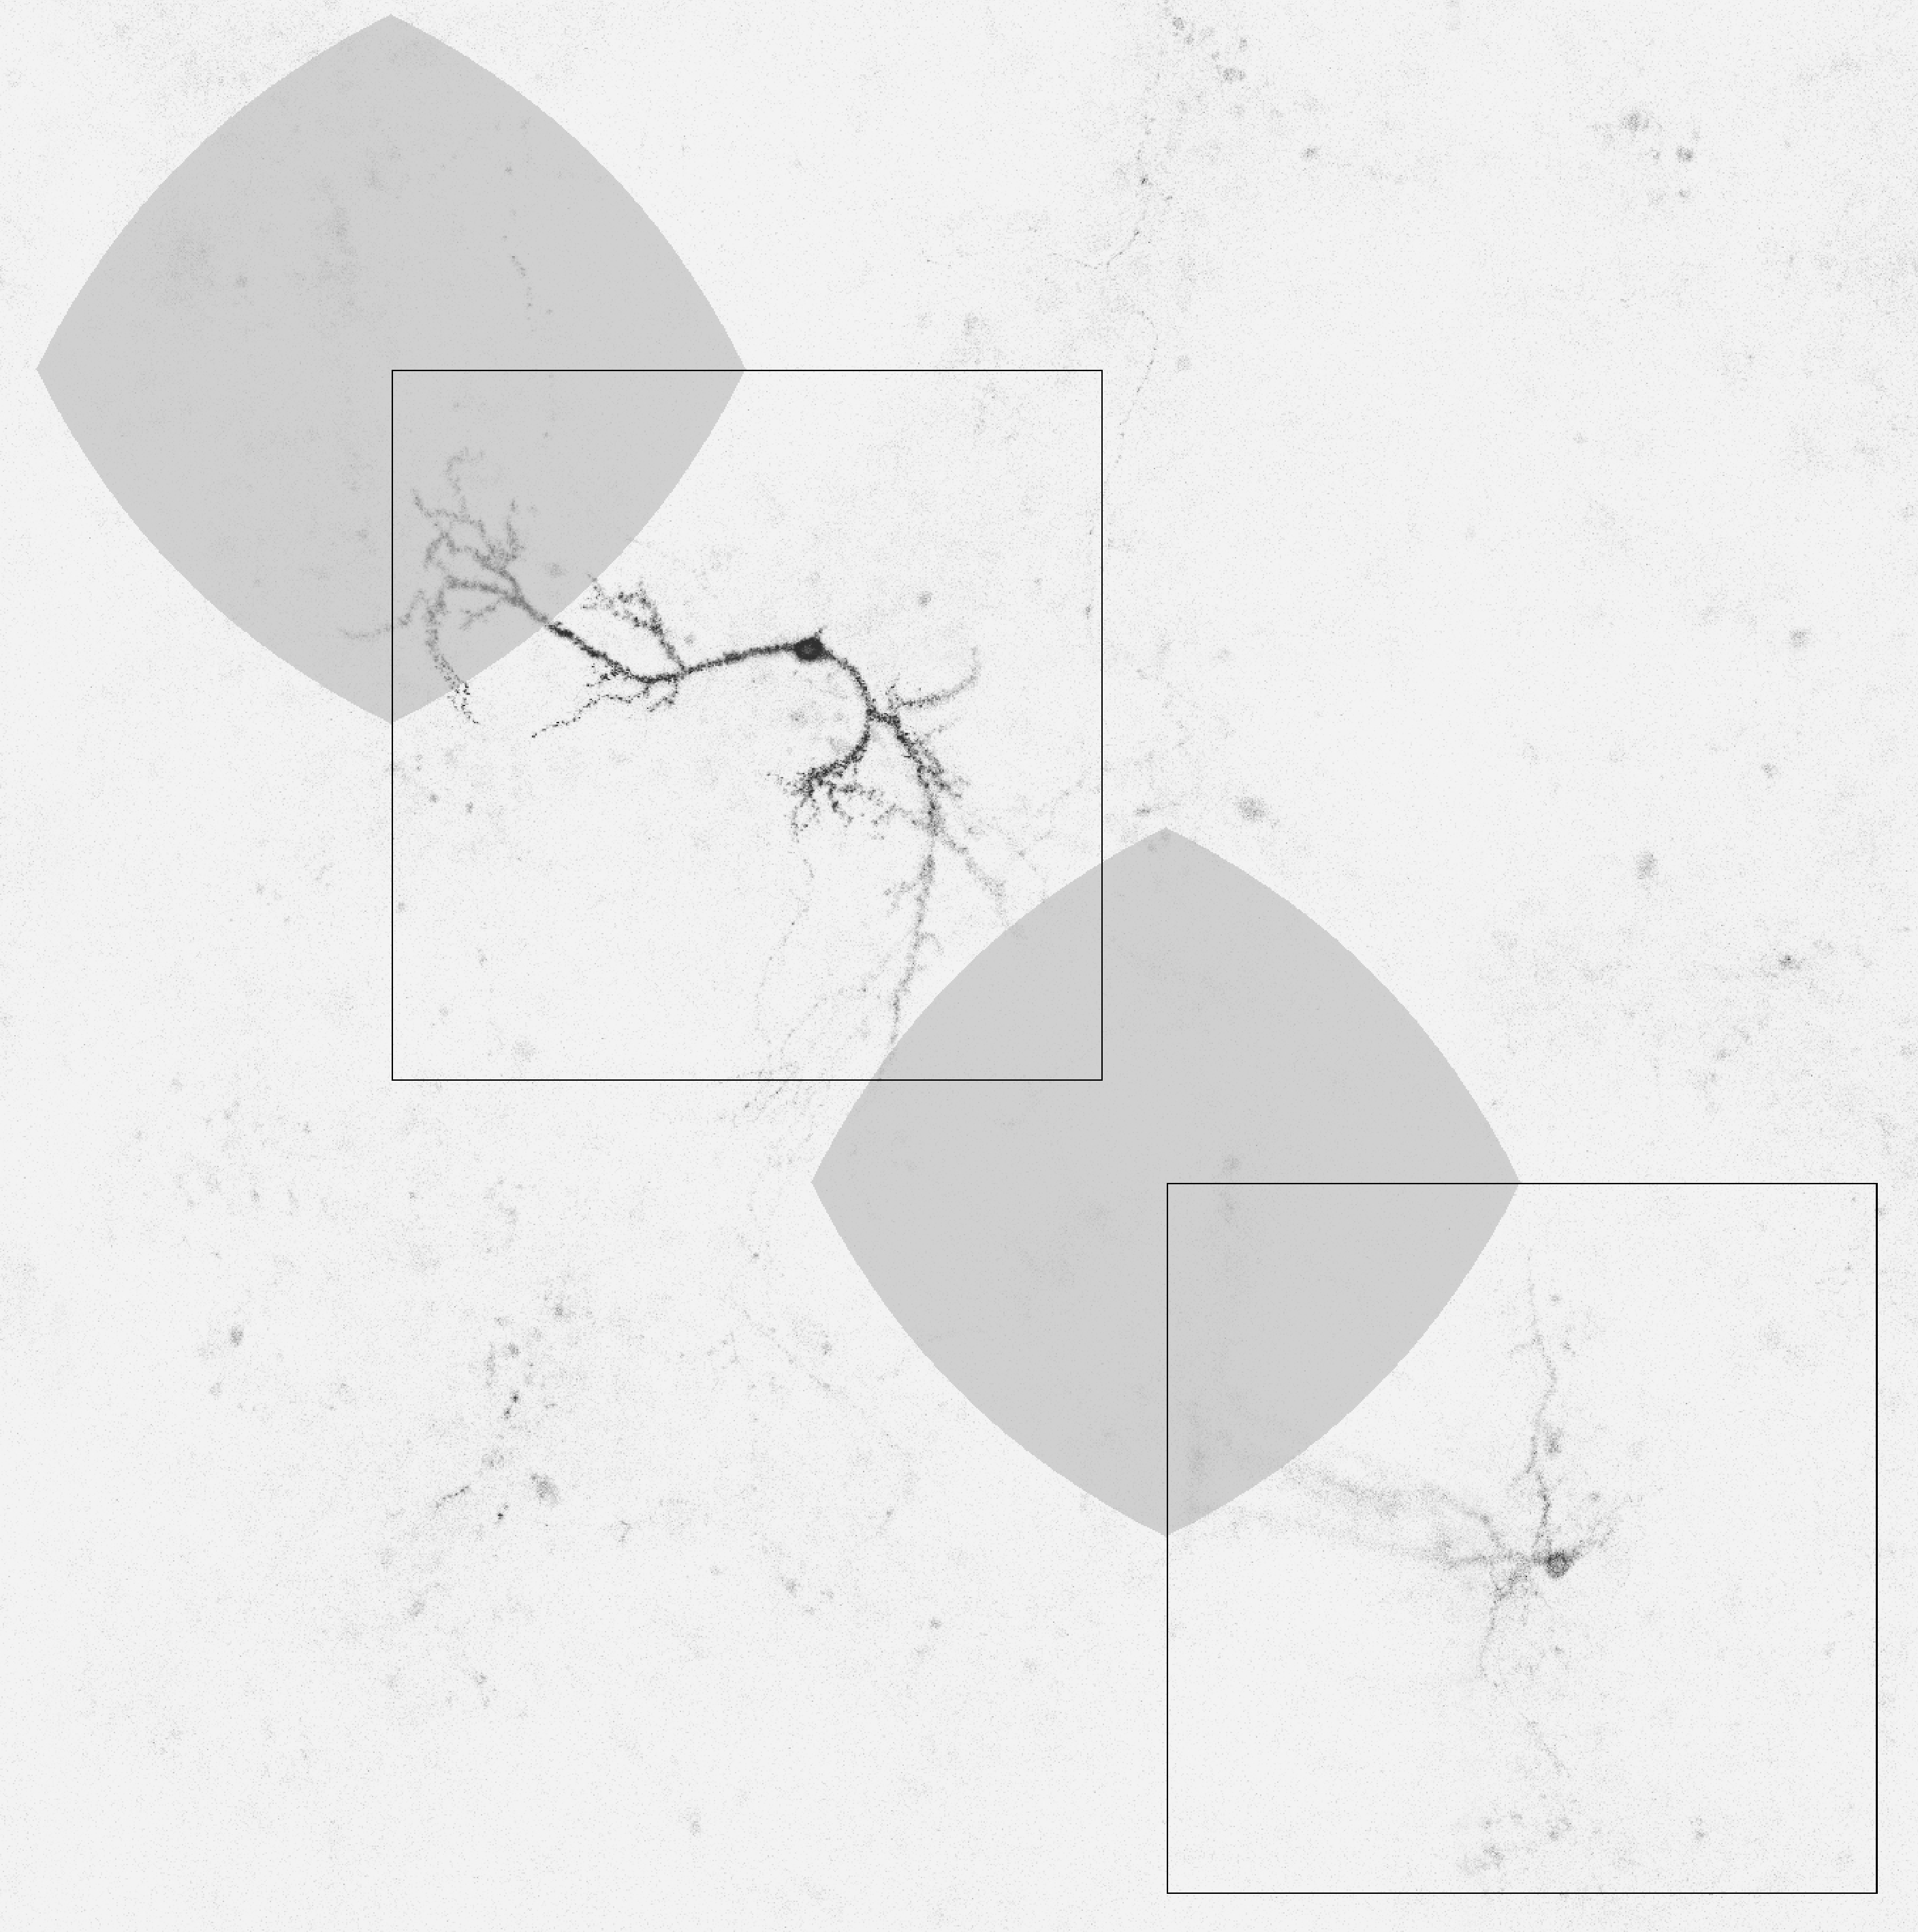
\includegraphics[width=\textwidth]{fig02}
	\end{minipage}
	\hspace{0.02\textwidth}
	\begin{minipage}{0.65\textwidth}
		\caption{Two example neurons with their expert-marked ROIs (black squares) and their potential alternative positive patch locations (gray regions). The latter comprise all possible top-left corner positions of patches with the same size as the given ROI and having 50\% or more area overlap with that ROI.}
		\label{ch5_fig2}
	\end{minipage}
\end{figure}
\subsection{Images features}
\label{subsec:imageFeaturesExtraction}
To train the machine learning algorithms, a large number of predefined features extracted from the positive and negative image patches is used. In this study two very comprehensive feature extraction approaches were employed: the compound hierarchy of algorithms representing morphology (CHARM) and the scale-invariant feature transform (SIFT). Each of them is briefly described in this section. In the training stage of the machine learning algorithms, feature values were normalized to zero mean and unit variance per feature over the whole data set, and constant features were pruned.

\subsubsection{CHARM features}
\label{subsubsec:wnd-chrm}
For the extraction of the CHARM features, the open-source software library WND-CHARM \cite{shamir2008wndchrm, orlov2008wnd} is used, which has been successful for many pattern recognition applications in biology \cite{shamir2010pattern, uhlmann2016cp} as well as in astronomy \cite{shamir2012automatic, kuminski2014combining} and in art \cite{shamir2012computer}. It can extract a large number of generic image descriptors and also includes a classifier based on the weighted neighbor distance (WND) between feature vectors. However, since the performance of this classifier was rather limited in the initial results of this study \cite{mata2016automatic}, alternative machine learning algorithms were explored for specified classification task, but using the image features calculated using this software library. In total 1,059 CHARM features are calculated for each positive and negative patch (recent versions of WND-CHARM can extract even more features but at an increased computational cost).

The calculated image features can be divided into four categories: polynomial decompositions, high-contrast features, pixel statistics, and texture descriptors. The first category includes features based on the Zernike polynomials and Chebyshev polynomials \cite{gradshteyn2014table} as well as Chebyshev-Fourier statistics. Features from the second category include various statistics calculated from the Prewitt edges \cite{prewitt1970object}, Gabor wavelets \cite{gabor1946theory}, and object masks obtained by Otsu thresholding \cite{otsu1979threshold}. The third category consists of image features calculated from the multiscale intensity histogram \cite{hadjidemetriou2001spatial} and various statistics based on the image moments. The last category includes the Haralick \cite{haralick1973textural} and Tamura \cite{tamura1978textural} texture features. In addition, the software calculates various image transforms, including the Radon, Fourier, wavelet, Chebyshev, and edge transforms, as well as transforms of image transforms. For more detailed technical descriptions of all features and transforms, reader is referred to \cite{orlov2008wnd}.

\subsubsection{SIFT features}
\label{subsubsec:sift-and-bow}
The SIFT algorithm \cite{lowe2004distinctive} is another popular method which extracts meaningful features from images for pattern recognition tasks. It has been used for a very wide range of applications in thousands of studies, including in biomedical image analysis \cite{ni2009reconstruction, jiang2010live, mualla2013automatic, zhang2013nonrigid, ni2009reconstruction, yu2016fast}. The extraction of SIFT features from a patch consists of four main steps. First, a Gaussian scale space is calculated, and potentially interesting points are identified by searching over all scales and locations for extrema in the difference-of-Gaussian function. Next, key points are selected from this list of candidates based on their measures of stability, and their precise location and scale are determined by model fitting. Then, based on the local gradient directions, each key point is assigned to one or more orientations (binned angles). And lastly, orientation histograms are constructed from the local gradients in a region around each key point, relative to the key point's assigned orientation, and the histogram entries constitute the elements of a (typically 128-dimensional) feature vector. Normalizing the feature vector results with a key point descriptor that is relatively invariant to spatial distortions and changes in illumination. All key point descriptors of a patch taken together form the SIFT features of that patch.

A problem in comparing image patches based on their SIFT features is that the number of key points, and thus the number of descriptors, may be different for each patch. The comparison is facilitated by applying a transform that represents each patch by a feature vector of fixed length \cite{yang2009linear}. A very effective and popular approach to achieve this is to use the bag-of-words (\gls{bow}) model \cite{fei2005bayesian}. Here, all descriptors of all available patches are divided into a fixed number of clusters by $k$-means clustering \cite{macqueen1967some}, and the mean of each cluster represents a visual `word', a vector of the same dimensionality as the descriptors. Subsequently, for any given patch, each of its descriptors is assigned to the single cluster to which it is closest according to the Mahalanobis distance. Such mapping yields a histogram vector of fixed length $k$, with each vector element being the number of patch descriptors assigned to the corresponding cluster.

To obtain the SIFT-BoW feature vector for each positive and negative patch, the VLFeat software library \cite{vedaldi2010vlfeat} is used in conjunction with MATLAB (The MathWorks Inc.). The vector length is a user parameter, and the classification performance of the different machine learning algorithms is evaluated for lengths of 20, 40, 60, 80, 100, 150, 200, and 230.

\subsection{Machine learning}
\label{subsec:machineLearning}
Four different machine learning algorithms were considered for the classification task in this study. This section summarizes the algorithms and their hyperparameters, explains the resampling strategies used in the training and testing of the algorithms, and the feature selection approach.
\begin{figure}[h!]
	\centering
	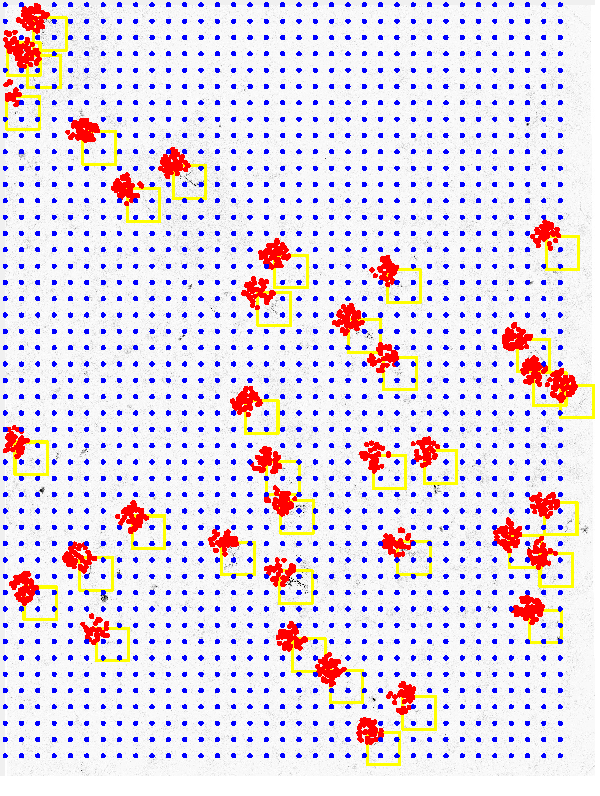
\includegraphics[width=0.8\columnwidth]{fig03}
	\caption{Example of positive patch oversampling. The background shows a high-content fluorescence microscopy image (with intensities inverted), and the graphical overlay shows the neuron ROIs marked by the expert (yellow squares), the top-left corners of the patches randomly sampled from all possible patches considered as alternative positives (red dots), and the intersection points (blue dots) of the regular grid used for negative patch sampling (Section~\ref{sec:annotation}).}
	\label{ch5_fig3}
\end{figure}
\subsubsection{Classification algorithms}
\label{subsubsec:classifiers}
{\bf Support Vector Machines} (SVM) are one of the best known and most successful machine learning algorithms for both classification and regression problems \cite{boser1992training, vapnik1998statistical, vapnik2013nature, bishop2006pattern}. In classification problems, the principal aim of SVM is to find the hyperplane in the feature space that best separates the given samples (in this case neuron and non-neuron patches), by maximizing the distance between the samples and the hyperplane \cite{burges1998tutorial}. If the problem requires more complex (nonlinear) separation functions, SVM can still be used, by employing so-called kernel functions that transform the high-dimensional feature space such that a hyperplane (linear) can still be used as the separation function. Generally speaking, one could interpret a kernel as a similarity measure \cite{vert2004primer}. Different types of kernels have been proposed, the Gaussian radial basis function (RBF) being one of the most popular \cite{cristianini2000introduction}. Two hyperparameters need to be optimized for best performance, one related to the SVM algorithm itself, the other related to the Gaussian RBF kernel. The first (`cost') is the trade-off between the misclassification of the samples and the simplicity of the decision surface. The second (`gamma') is the free parameter of the Gaussian function. The grid search used in the experiments of this study considers values $2^k$ for integer $k=-12,\dots,12$ for both parameters.

{\bf Random Forest} (\gls{rf}) is another prominent machine learning algorithm for classification and regression \cite{breiman2001random}. As a classifier, it operates by randomly taking multiple bootstrapped subsets of the data, fitting a decision tree to each one of them, and outputting the mode of the class outputs of the individual trees. This approach reduces the possibility of overfitting the training dataset and generally produces more accurate results than a single decision tree. The RF has two main hyperparameters. The first (`node size') is the minimum size of the terminal nodes of the decision trees. Throughout the experiments, integer values of 1\dots5 were considered for this parameter. The second (`mtry') is the number of features randomly sampled as possible candidates at each split. For this parameter, integer values of 5\dots36 were considered.

{\bf k-Nearest Neighbor} (\gls{knn}) classification operates by comparing an unclassified patch to patches with known class labels (the reference set), then selecting the k most similar of these patches (the nearest neighbors) according to some distance metric in the feature space, and outputting the most frequently occurring class label of these patches \cite{cover1967nearest}. In this study, a weighted KNN algorithm is used \cite{hechenbichler2004weighted, samworth2012optimal} which employs the Minkowski distance and classifies patches using the maximum of summed kernel densities. This algorithm uses kernel functions to weigh the neighbors according to their distances. The KNN algorithm requires optimization of only one hyperparameter (`k'), for which integer values of 3\dots9 are considered.

{\bf Generalized Linear Model} (\gls{glmnet}) via penalized maximum likelihood \cite{friedman2010regularization} is a regularized statistical model whose response variable is a Bernoulli indicator used for classification. It is based on the least absolute shrinkage and selection operator (\gls{lasso}) \cite{tibshirani1996regression}. Similar to the LASSO, this method simultaneously performs automatic feature selection and continuous shrinkage (regularization), and is able to select groups of correlated features. Specifically, GLMNET combines $l_1$ and $l_2$ penalties for regularization, and has two hyperparameters. The first (`alpha') is in the range $[0,1]$ and linearly weighs the contributions of the different types of penalities, with value 0 corresponding to $l_2$ regularization, and 1 to $l_1$ regularization. Throughout the experiments, values 0, 0.15, 0.25, 0.35, 0.5, 0.65, 0.75, 0.85, and 1 were used. The second parameter (`lambda') determines the degree of regularization, for which values of 0.0001, 0.001, 0.01, 0.1, and 1 were considered.

The statistical computing software tool R \cite{team2016vienna} was used in the conducted experiments along with the R packages \textit{mlr} \cite{bischl2016mlr}, \textit{e1071} \cite{meyer2017e1071}, \textit{random-Forest} \cite{liaw2002classification}, \textit{kknn} \cite{schliep2016kknn}, and \textit{GLMnet} \cite{friedman2010regularization}, to evaluate all the machine learning algorithms. Most of the result plots presented in this chapter were generated using the R package \textit{ggplot2} \cite{wickham2009ggplot2}.
\begin{figure}[h!]
	\centering
	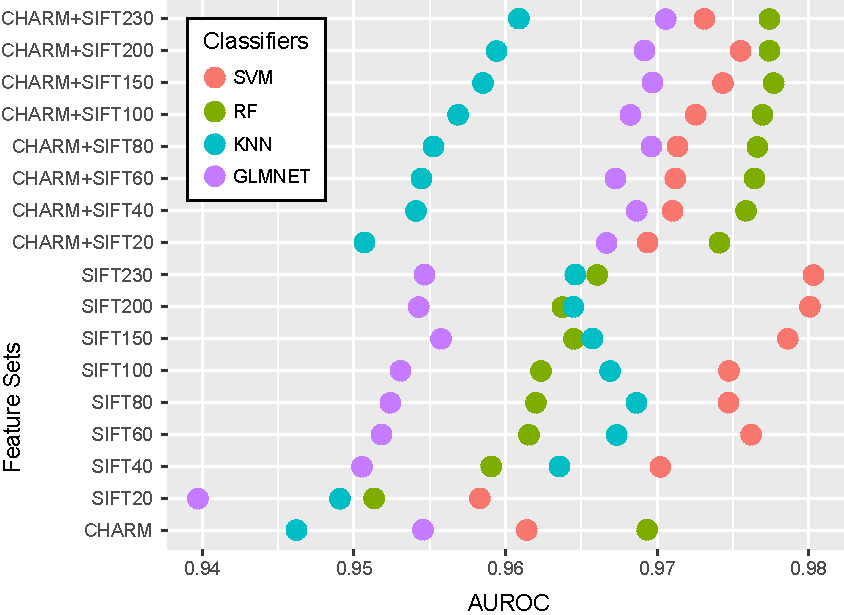
\includegraphics[width=0.9\columnwidth]{fig04}
	\caption{Results of the initial exploratory experiment. Each of the considered classifiers (SVM, RF, KNN, GLMNET) was evaluated for each of the described 17 feature sets according to the performance measure (AUROC) using the described simplified resampling strategy.}
	\label{ch5_fig4}
\end{figure}
\subsubsection{Resampling strategies}
\label{subsubsec:resampling}
The mentioned hyperparameters of the machine learning algorithms need to be optimized for best performance. To accomplish this, and at the same time make an honest comparison of the algorithms under equal conditions, a nested resampling approach \cite{simon2007resampling, bischl2012resampling} is used, involving an inner loop and an outer loop. In this approach, the actual performance assessment of the algorithms takes place in the outer loop, implemented as three independent runs of a 10-fold cross-validation experiment, with stratification (to ensure having the same proportion of positive and negative samples in all partitions of the cross-validation), where the final performance scores are obtained by aggregation. In each iteration of the outer loop, the corresponding training set is used in an inner loop, to find the optimal values of the hyperparameters of the algorithms. The inner loop was implemented using a holdout approach, where the given training set from the outer loop is redivided into a training subset (2/3rd of the set) and a validation subset (1/3rd of the set), and a grid search is run on the hyperparameters. The hyperparameter values that give the best performance are subsequently used to retrain the algorithms on the given training set from the outer loop. This nested resampling strategy is statistically sound but computationally expensive. To make the experiments computationally feasible, the search space is discretized using the hyperparameter values listed in the previous section.

\subsubsection{Feature selection}
\label{subsubsec:featureSelection}
Although a priori it is appropriate to consider as many features as possible, and increasing  computational power allows us to construct larger and larger feature sets, in the end many features may be irrelevant or may even negatively impact the performance of the machine learning algorithms. Thus the experimentation also aimed to investigate which of all considered features positively contribute most to the performance of the algorithms in this application. Knowledge of the best features allows one to build potentially better and computationally more efficient classifiers. Moreover, it may shed light on which image information is most relevant to the classification task, which in turn may provide useful hints to improve the imaging process. There exist various approaches for feature selection using machine learning algorithms in supervised classification problems, including filter, wrapper, and embedded approaches \cite{saeys2007review}. This study uses the filter approach, as it is independent of the classifier, fast, scalable, and needs to be applied only once, after which the different algorithms can be evaluated.
\section{Experimental results}
\label{ch5:sec:experimental-results}
All experiments in this study were carried out using the BioCAI HPC cluster facility at the University of A Coru\~{n}a. The area under the receiver operating curve (AUROC) measure is used to quantitatively assess and compare the performances of the machine learning algorithms as it captures both Type I and Type II errors \cite{fawcett2006introduction}. First, an initial exploratory experiment was performed on various combinations of CHARM and SIFT feature sets to find out which of these deserved closer investigation. An in-depth performance evaluation of all the algorithms was conducted using the most promising feature sets, subsequently investigating which specific features of the complete set contributed most to the performance. Finally, an analysis was made to see whether the differences in performance of the algorithms were statistically significant or not.
\begin{figure}[h!]
	\centering
	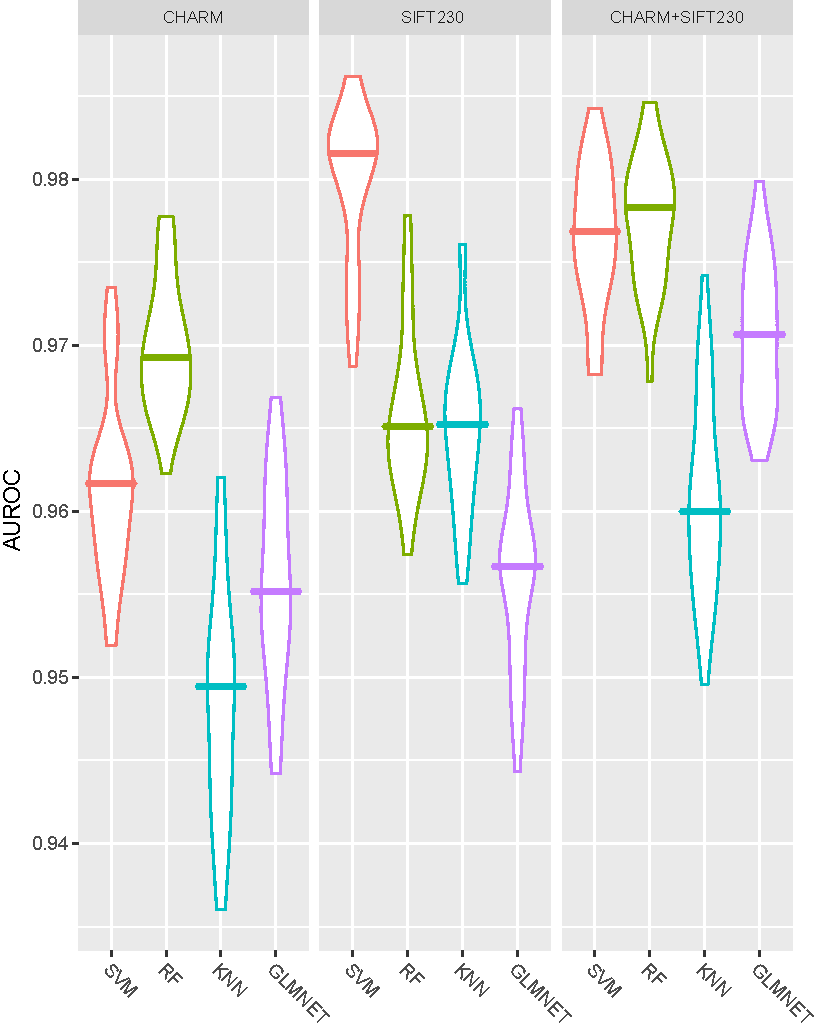
\includegraphics[width=0.9\columnwidth]{fig05}
	\caption{Results of the cross-validation experiment. Each of the considered classifiers (SVM, RF, KNN, GLMNET) was evaluated for each of the selected feature sets (CHARM, SIFT230, CHARM+SIFT230) using the performance measure (AUROC). The results are shown as violin plots, where the horizontal bar indicates the median value, the vertical extent is the interquartile range, and the width indicates the estimated probability density.}
	\label{ch5_fig5}
\end{figure}
\subsection{Initial exploratory results}
\label{subsec:initialExploratoryExperiments}
For the initial experiment 17 different feature sets were constructed from (combinations of) the CHARM features and the SIFT features: CHARM features only (one set), SIFT features only (eight sets, one for each of the eight BoW vector lengths), and the union of CHARM and SIFT features (eight sets). To avoid prohibitive computation times in the cross-validation experiment (described next), it was first explored which of these feature sets would likely yield the best classification results with the considered machine learning algorithms. The feature sets were preprocessed by normalizing each feature to zero mean and unit standard deviation over all patches, and removing constant features (if present), to reduce the effect of possible outliers. To make this exploratory experiment more computationally feasible, a simpler resampling strategy was used rather than the described one, namely a single 10-fold cross-validation in the outer loop, and a holdout approach in the inner loop. In the latter, the optimal hyperparameters of the classification algorithms were obtained using a grid search on 2/3rd of the training set of the outer loop, and validated on the remaining 1/3rd.
\begin{figure}[ht]
	\centering
	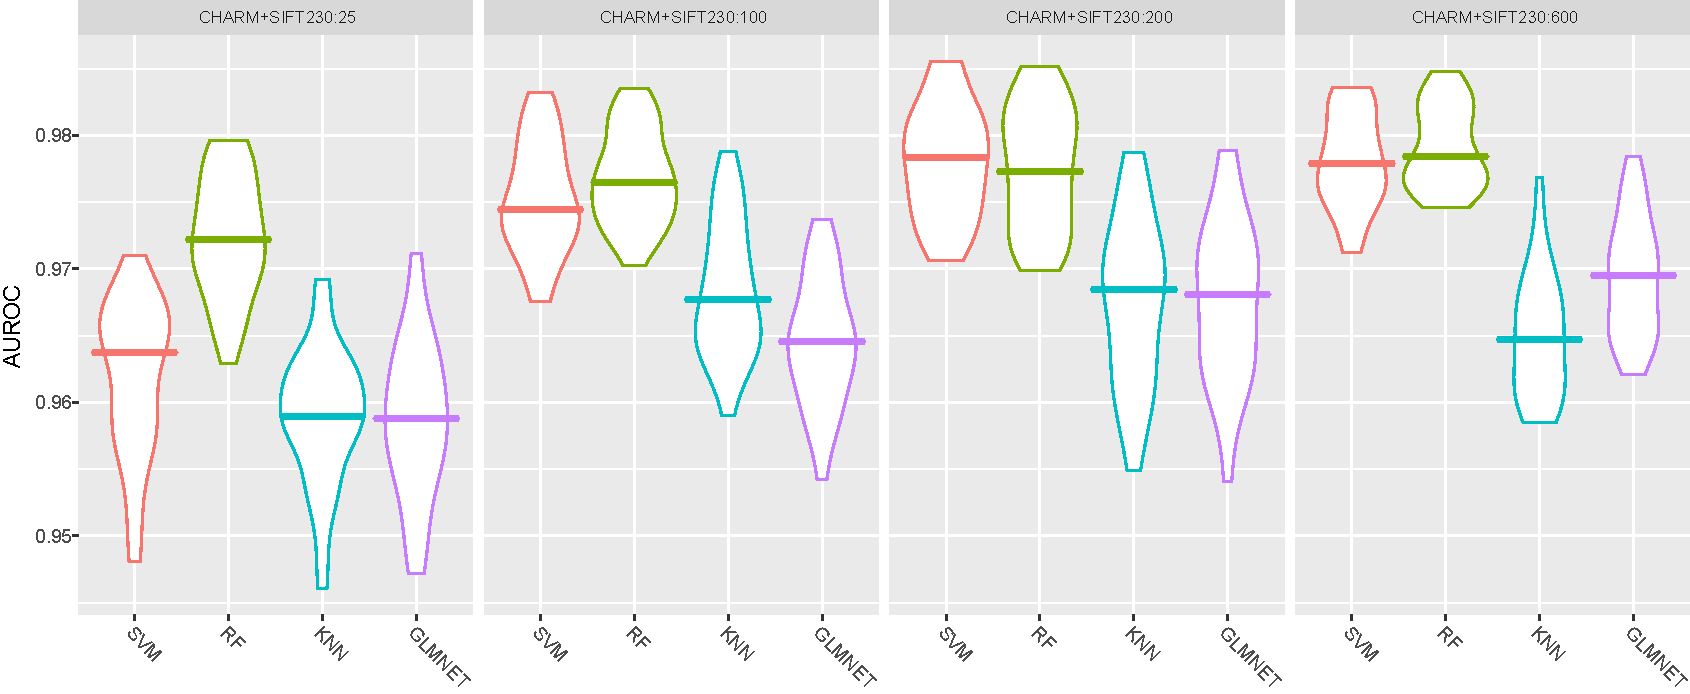
\includegraphics[width=\textwidth]{fig06}
	\caption{Performance (AUROC) of the considered classifiers (SVM, RF, KNN, GLMNET) for different feature subsets (the top 25, 100, 200, and 600 features from the CHARM+SIFT230 set). The results are shown as violin plots, where the horizontal bar indicates the median value, the vertical extent is the interquartile range, and the width indicates the estimated probability density.}
	\label{ch5_fig6}
\end{figure}
Observing the results (Fig.~\ref{ch5_fig4}) indicates that both the absolute and the relative performance of the classifiers was quite different for the different feature sets. Specifically, for SVM and KNN, the best results were obtained with the SIFT features alone (for sufficiently large BoW vector lengths), while the CHARM features alone produced inferior results, and with the combination of CHARM and SIFT features these classifiers performed somewhere in between. For RF and GLMNET, on the other hand, the SIFT features alone yielded inferior results, and with the CHARM features alone these classifiers did not fare much better, but the combination of CHARM and SIFT features (for all BoW vector lengths) produced the best results.

Thus it was concluded that the cross-validation experiment should include both the CHARM and SIFT feature sets alone, as well as their combination, and the only way to reduce the computational cost of that experiment was to select a specific SIFT-BoW vector length. Overall, the results seemed to indicate that in most cases it is better to use larger vector lengths, and simply taking the maximum considered length (230) is a good choice.
\begin{figure}[h!]
	\centering
	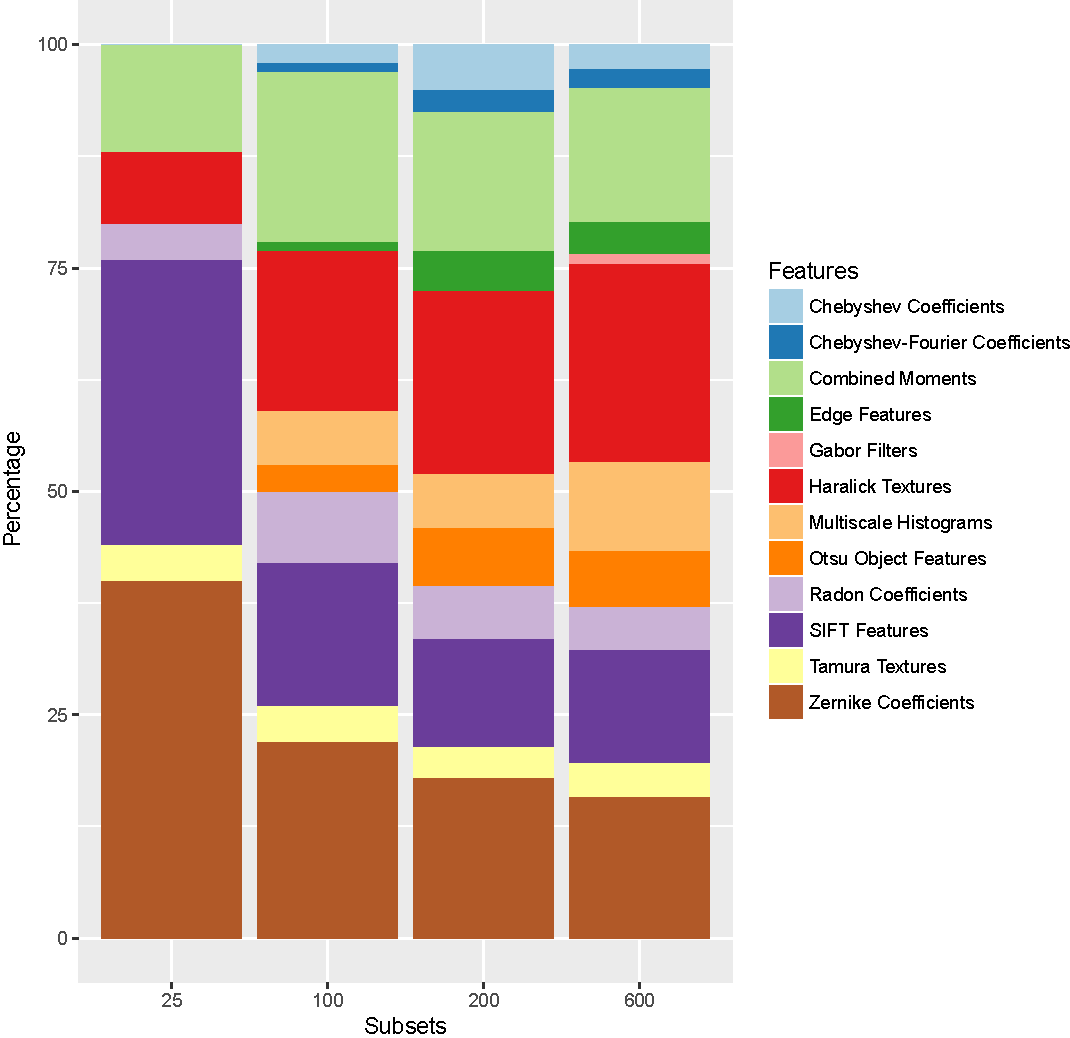
\includegraphics[width=\columnwidth]{fig07}
	\caption{Cumulative percentages of the different types of features contained in the four subsets (the top 25, 100, 200, and 600 features selected from the CHARM+SIFT230 set).}
	\label{ch5_fig7}
\end{figure}
\subsection{Cross-validation results}
\label{subsec:baselineResults}
Based on the results of the initial exploratory experiment three feature sets corresponding to CHARM features only, SIFT230 features only, and CHARM+SIFT230 features are selected to evaluate the four machine learning classifiers using a cross-validation experiment, involving an outer loop (3 $\times$ 10-fold) for performance assessment and an inner loop (holdout) for hyperparameter optimization as described. The results (Fig.~\ref{ch5_fig5}) show that virtually all classifiers achieved AUROC values of $>$95\% and, generally, SVM and RF outperformed KNN and GLMNET. Considering the different feature sets, it is observable that all classifiers except RF achieved better performance with the SIFT230 feature set than with the CHARM feature set. This is interesting since the latter is much more extensive (1,059 features of many different types) than the former (230 BoW clusters). Apparently the SIFT230 features are more descriptive of the image content in showcased application. This is confirmed by the results with the CHARM+SIFT230 feature set, which are consistently better than with the CHARM feature set alone. However, whereas RF and GLMNET performed best using the more extensive CHARM+SIFT230 set, SVM and KNN performed best using the SIFT230 set alone. Overall, the best results were obtained with the SVM classifier using the SIFT230 feature set, although SVM and RF using the combined CHARM+ SIFT230 features performed comparably (statistical significance is discussed in Section~\ref{subsec:experimentalAnalysis}).
\subsection{Feature selection results}
\label{subsec:featureSelectionResults}
Next, the complete CHARM+SIFT230 feature set was subjected to a feature selection experiment. Specifically, the aim was to find out which features contributed most to the performance of the different classifiers, and whether these features alone could yield similar or even better classification performance than using the complete set, as that would make the classification task computationally cheaper.
\begin{figure}[h!]
	\centering
	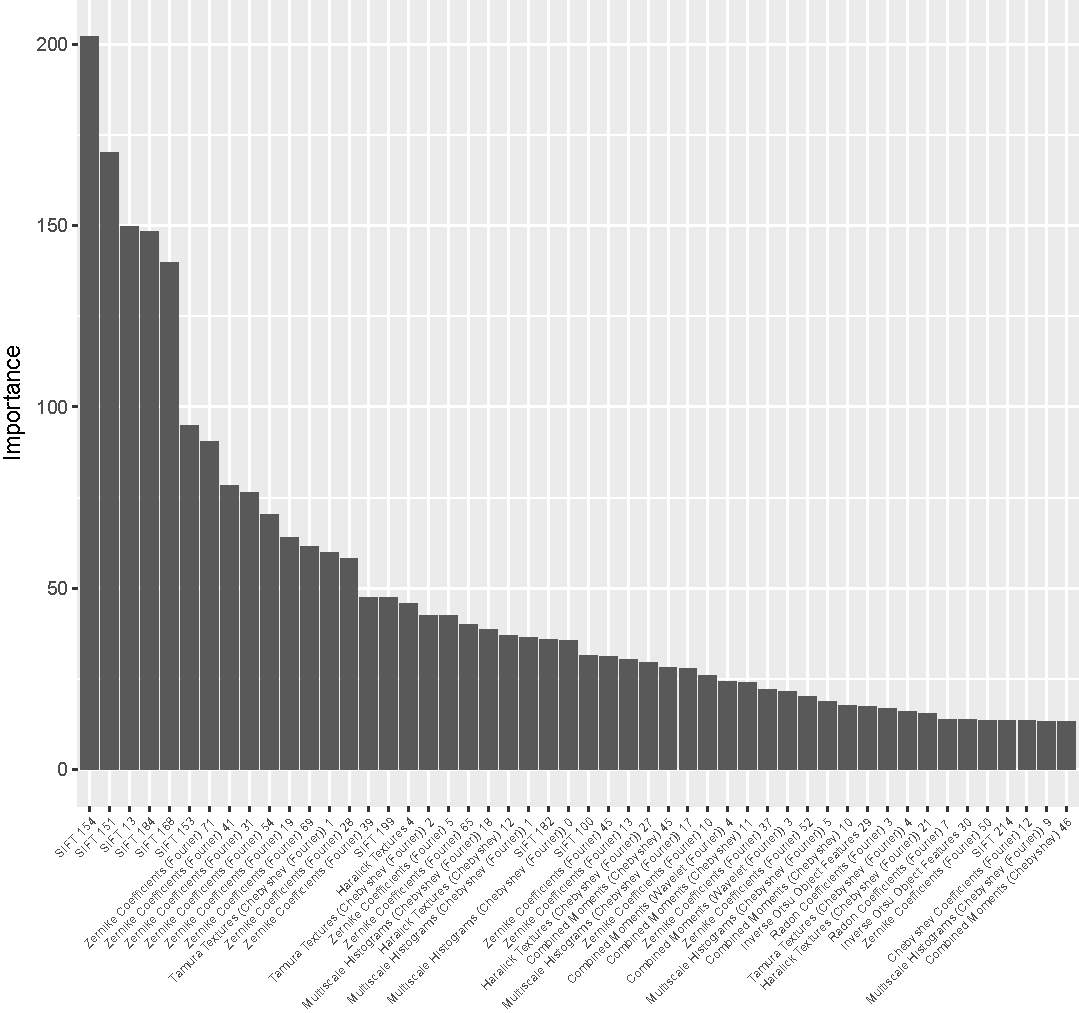
\includegraphics[width=\columnwidth]{fig08}
	\caption{The 50 most important features from the CHARM+SIFT230: 600 feature subset used by the best performing classifier. Importance was calculated according to the Gini index of the RF classifier. The importance value for each feature was averaged over all runs and folds of the cross-validation experiment.}
	\label{ch5_fig8}
\end{figure}
To this end, all 1,289 features are ranked using a \textit{CForest} test \cite{strobl2009party} and considered four subsets, consisting of the top 25, 100, 200, and 600 features. The results (Fig.~\ref{ch5_fig6}) agree with those of the previous experiment in that SVM and RF consistently outperformed KNN and GLMNET for all feature subsets. The results further indicate that the larger the number of top features, the better the performance of all four classifiers, but for most of them there was little improvement beyond the top 200 features. In fact, the scores of the best performing classifiers, SVM and RF, were very similar for the CHARM+SIFT230:200 subset and the full CHARM+SIFT230 set, and with smaller standard deviations (statistical significance is discussed in Section~\ref{subsec:experimentalAnalysis}). This indicates that the non-selected features provided noise rather than useful information to the classifiers.

Analyzing the types of features contained in the four subsets (Fig.~\ref{ch5_fig7}), indicates that the top 25 subset is dominated by the SIFT features and the Zernike coefficients from CHARM, whereas the top 100, 200, and 600 subsets include many other types of features (about twice as many), in roughly similar proportions. These additional features contribute important information to the classification process, as follows from the fact that the performance of the larger subsets is considerably better than that of the top 25 subset. However, it remains elusive why these specific types of features are dominant. According to the feature selection results (Fig.~\ref{ch5_fig6}), the best performing classification model is the RF using the CHARM+SIFT230:600 feature subset (AUROC = 0.9784), followed very closely by the SVM using the CHARM+SIFT230:200 feature subset (AUROC = 0.9783). Studying the importance of the features in the former model according to the \textit{Gini} index \cite{breiman2001random}, reveals (Fig.~\ref{ch5_fig8}) that the most important features are indeed from the SIFT set together with the Zernike coefficients from the CHARM set. Other important top features from the CHARM set in decreasing order include the Tamura and Haralick textures, multiscale histograms, combined moments, and others (Fig.~\ref{ch5_fig7}).
\begin{figure}[ht]
	\begin{minipage}{0.65\textwidth}
	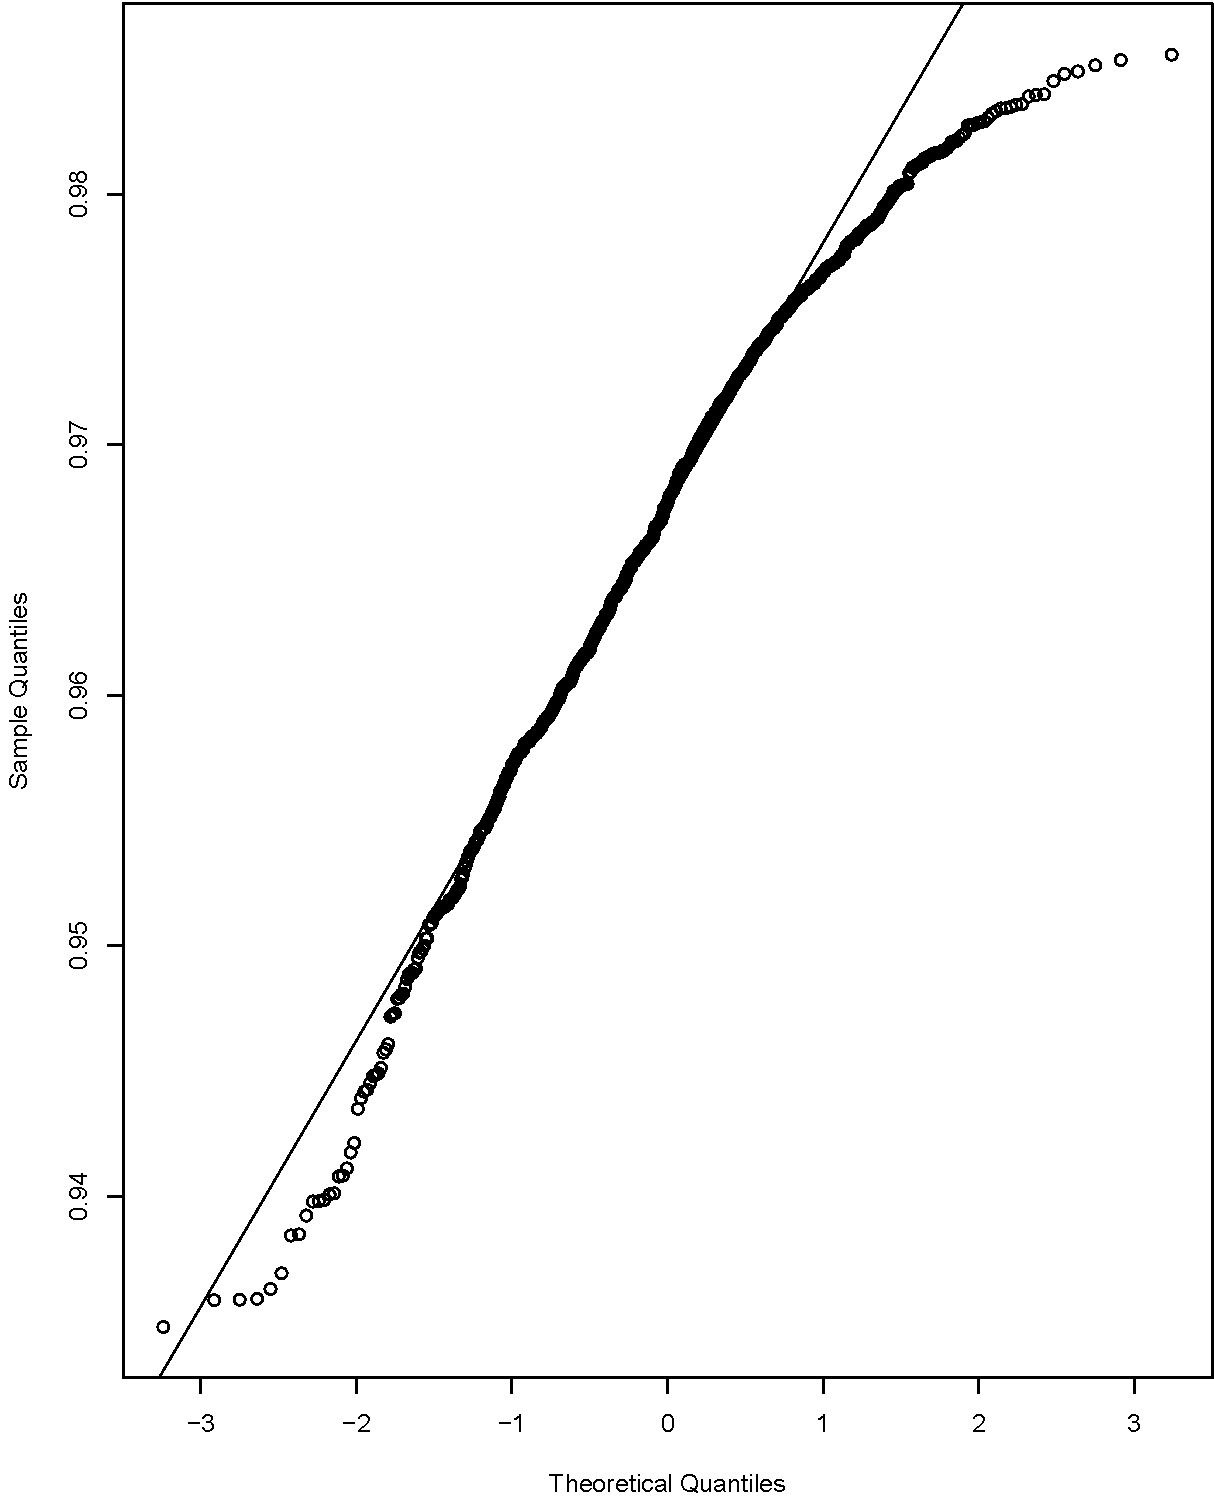
\includegraphics[width=\textwidth]{fig09}
	\end{minipage}
	\hspace{0.02\textwidth}
	\begin{minipage}{0.30\textwidth}
	\caption{Quantile-quantile (Q-Q) plot of the theoretical normal distribution and the data samples used. Clearly, the computed values (small circles) deviate substantially from a straight line (the solid line is the least squares fit) and reveal a nonlinear relationship, leading to the conclusion that the used data is not normally distributed.}
	\label{ch5_fig9}
	\end{minipage}
\end{figure}
\subsection{Statistical analysis results}
\label{subsec:experimentalAnalysis}
Finally the statistical significance of the results (AUROC values) of the considered classification algorithms on the selected feature (sub)sets was examined, to see if any particular model (combination of features and classifier with corresponding optimal hyperparameters) is to be preferred for this application. There exist mainly two types of statistical test to do this: parametric and non-parametric. Although parametric tests can be more powerful, they require normality, independence, and heteroscedasticity of the data \cite{fernandez2016methodology}. The first condition was checked using the Shapiro-Wilk test \cite{shapiro1965analysis} with the null hypothesis that the used data follows normal distribution, eventually rejecting the null hypothesis with very significant values of $W = 0.97324$ and $p < 2.723 \cdot 10^{-11}$ (see also the Q-Q plot in Fig.~\ref{ch5_fig9}). Since this already disqualifies parametric testing, there was no need to check the other conditions.
\begin{figure}[h!]
	\centering
	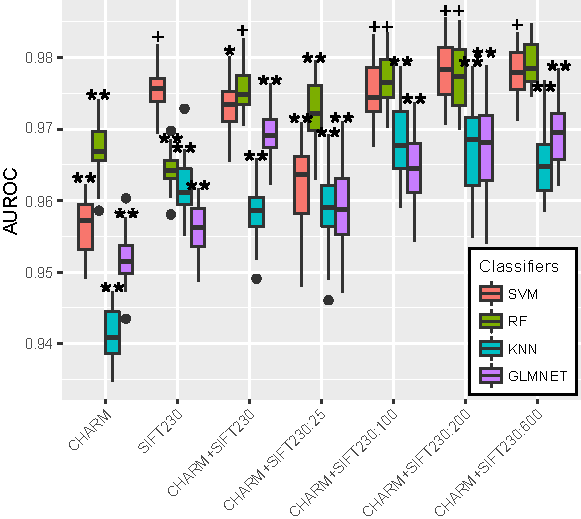
\includegraphics[width=0.65\columnwidth]{fig10}
	\caption{Results of the Friedman-Finner test showing the statistical significance of the differences in performance of the considered models (classifiers SVM, RF, KNN, and GLMNET, using any of the selected feature (sub)sets CHARM, SIFT230, CHARM+SIFT230, and the top 25, 100, 200, and 600 features of the latter) with respect to the control model (RF using CHARM+SIFT230:600). Performance values (AUROC) of each model from all runs and folds of the cross-validation experiment are summarized using the ggplot2 box plot. Significance with respect to the control model is indicated for $p > 0.05$ (+), and $0.01 < p < 0.05$ (*), and $p < 0.01$ (**).}
	\label{ch5_fig10}
\end{figure}
Thus a non-parametric test - the Friedman test \cite{friedman1940comparison} was used. It is known to yield conservative results in the case of relatively small numbers of algorithms and datasets \cite{garcia2010advanced}. The null hypothesis that all models yield the same performance on used data was rejected with very significant values of $\chi^2 = 657$ and $p < 2.25 \cdot 10^{-10}$. Since this means that at least some models are statistically significantly better or worse than others, subsequent examination tested for significant differences between all pairs of models using the post-hoc Finner test \cite{finner1993monotonicity}, with the control model being the RF classifier using the CHARM+SIFT230:600 feature set, as it performed best in the feature selection experiment (Fig.~\ref{ch5_fig6}).

The results (Fig.~\ref{ch5_fig10}) show that several other models performed statistically similar to the control model. These include the SVM classifier using the SIFT230 feature set or the top 100, 200, or 600 features of the CHARM+SIFT230 set. Other statistically similar models include the RF classifier using the CHARM+SIFT230 feature set, or just the top 100 or 200 features of the latter. None of the models based on the KNN and GLMNET classifiers performed statistically similar to the control model.

\section{Discussion and conclusions}
\label{sec:discussion}
The aim of the presented study was to find out which machine learning based classification algorithms and which commonly used feature extraction algorithms would be most suited for the task of detecting neurons in high-content fluorescence microscopy image data typically acquired in screening experiments. To this end, four popular classifiers (SVM, RF, KNN, GLMNET) and two popular feature extraction tools (CHARM and SIFT) were considered, and various experiments and statistical analyses performed to narrow down and compare the many possible models (combinations of classifiers and (sub)sets of features).

Showcased results point to the conclusion that of all considered classifiers, SVM and RF generally work best, provided they are fed with the right sets of features. Statistically similar performance was observed with the following models: SVM using SIFT (230 features), SVM using CHARM+SIFT (the top 100, 200, or 600 features), and RF using CHARM+SIFT (the full 1,289 features or only the top 100, 200, or 600 features). In the course of conducted study, the potential of several alternative features was also explored, such as the histogram of oriented gradients (\gls{hog}) \cite{dalal2005histograms} and spatial pyramid matching (\gls{spm}) \cite{lazebnik2006beyond} based on sparse coding (ScSPM) \cite{yang2009linear}, but the results were not as good.
\begin{figure}[ht]
	\centering
	\begin{tabular}{@{}c@{\hspace{0.02\textwidth}}c@{}}
		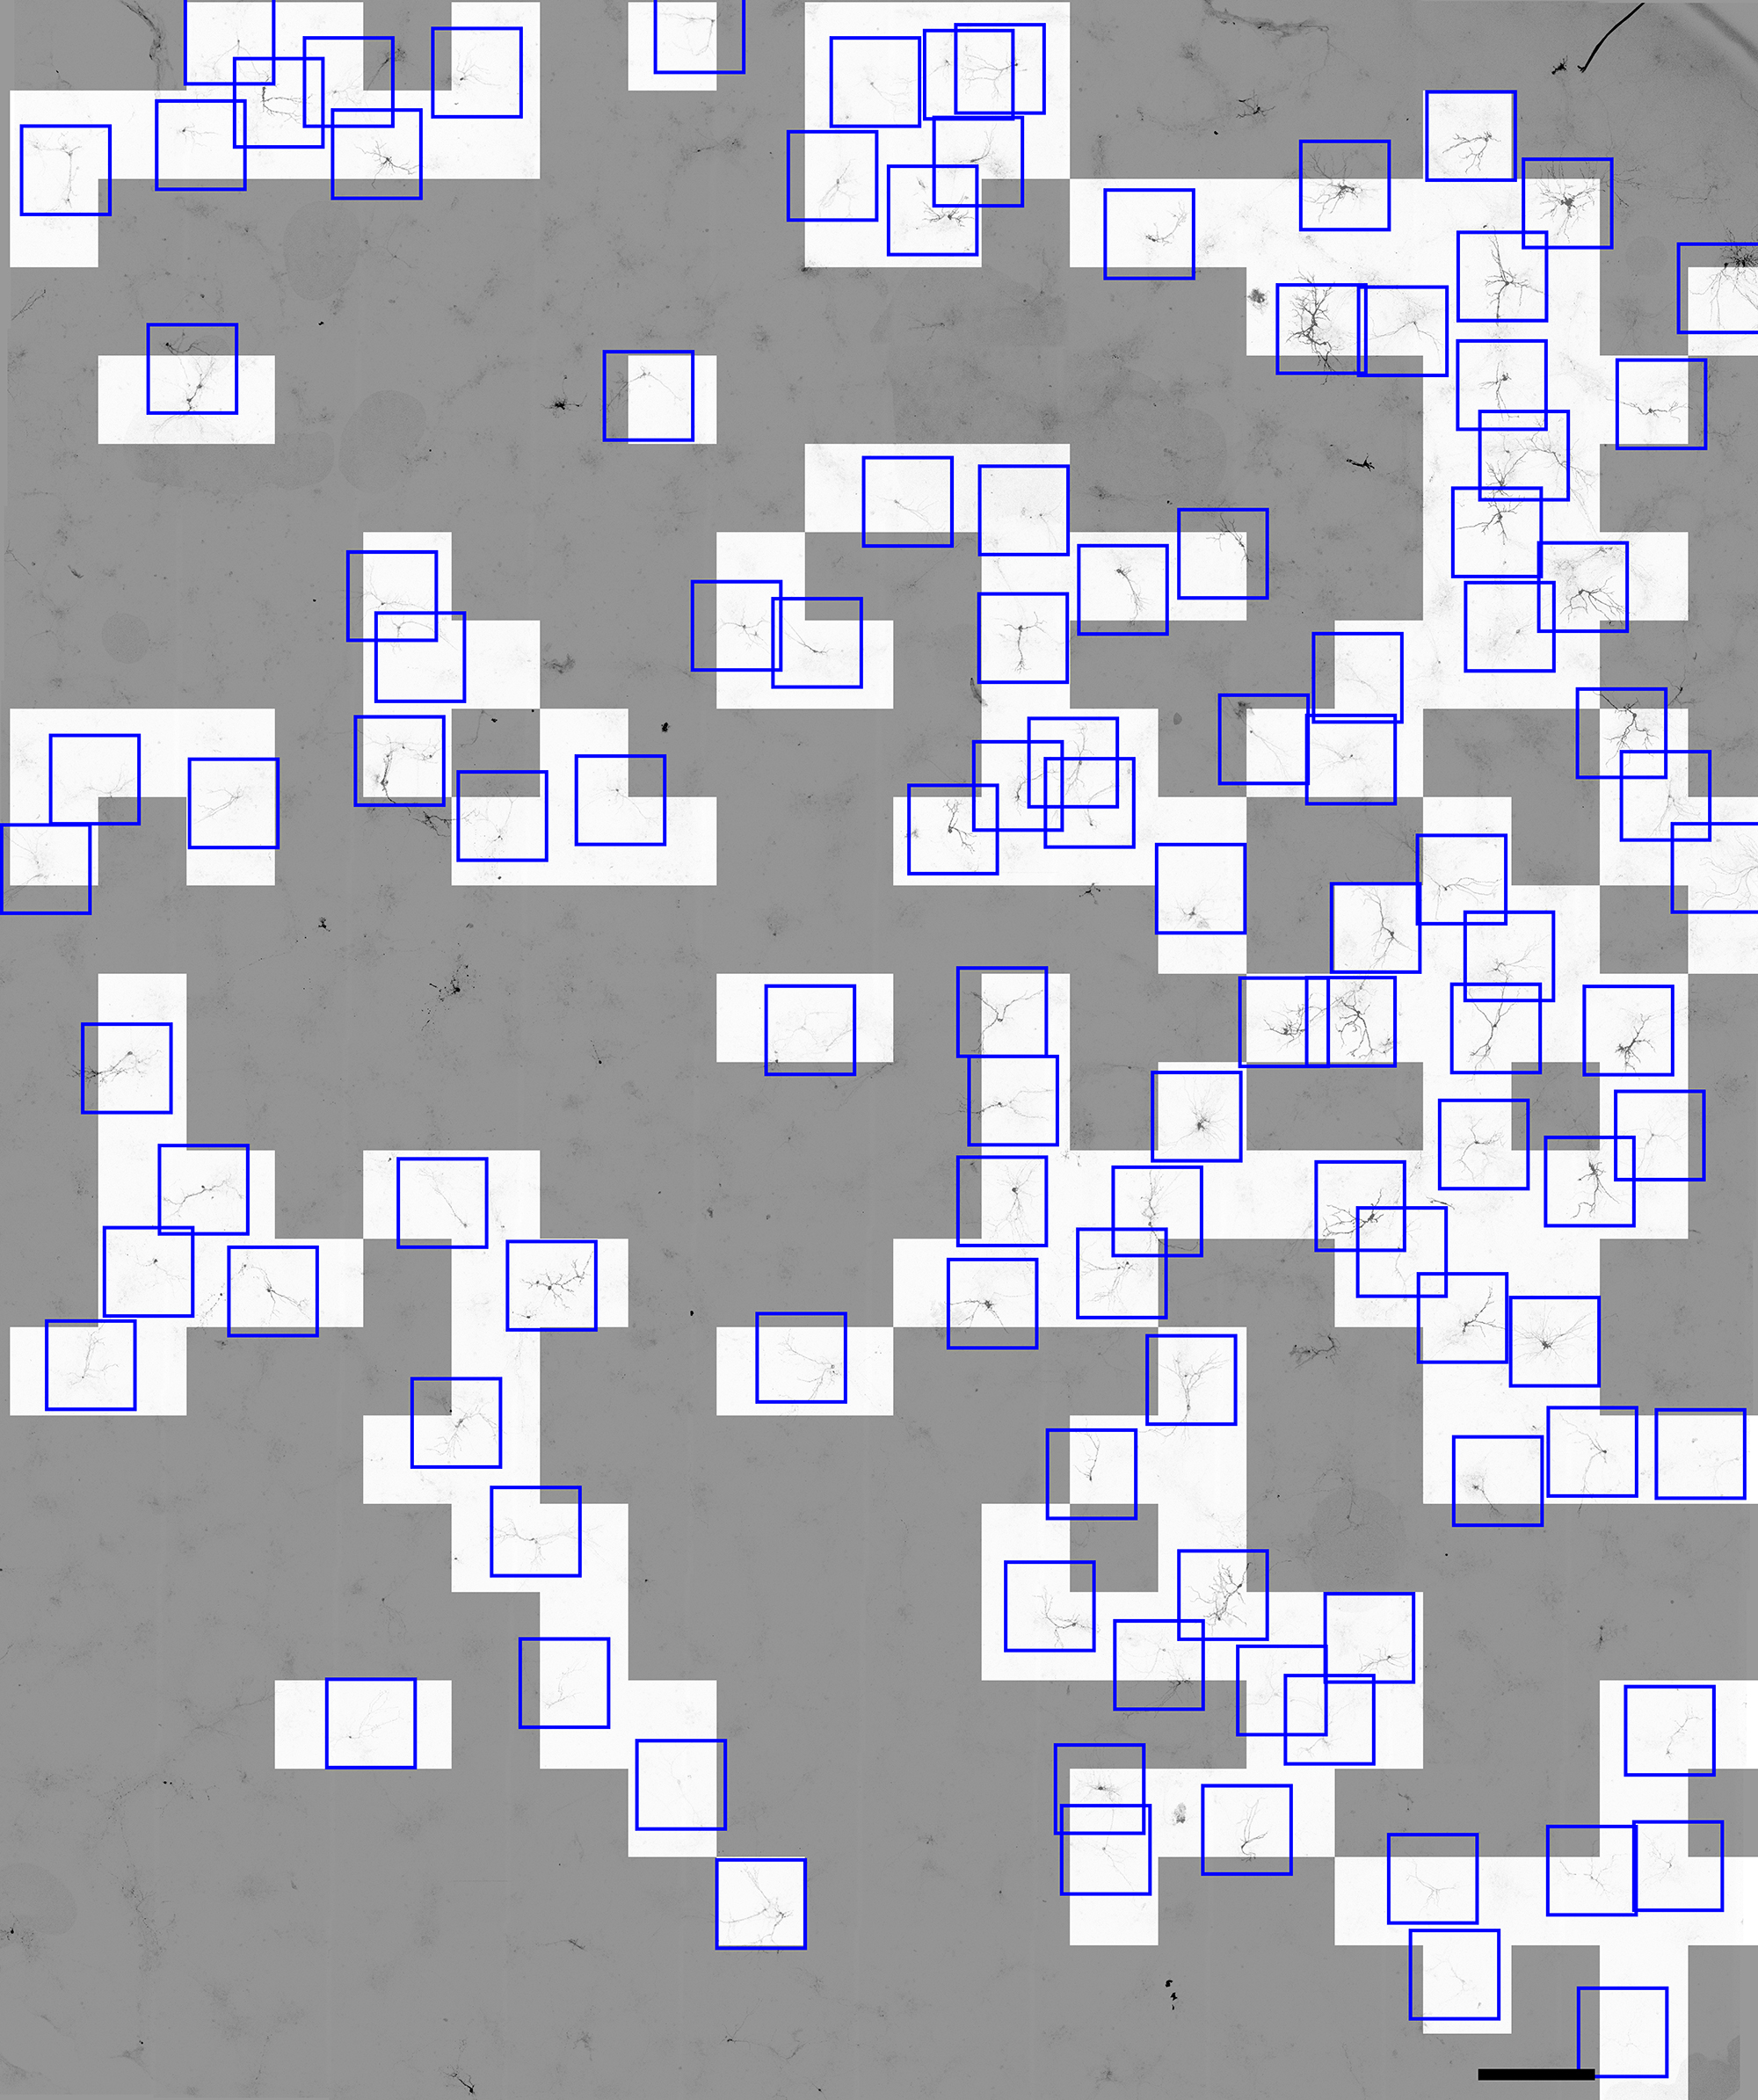
\includegraphics[height=0.50\textwidth]{fig11a} &
		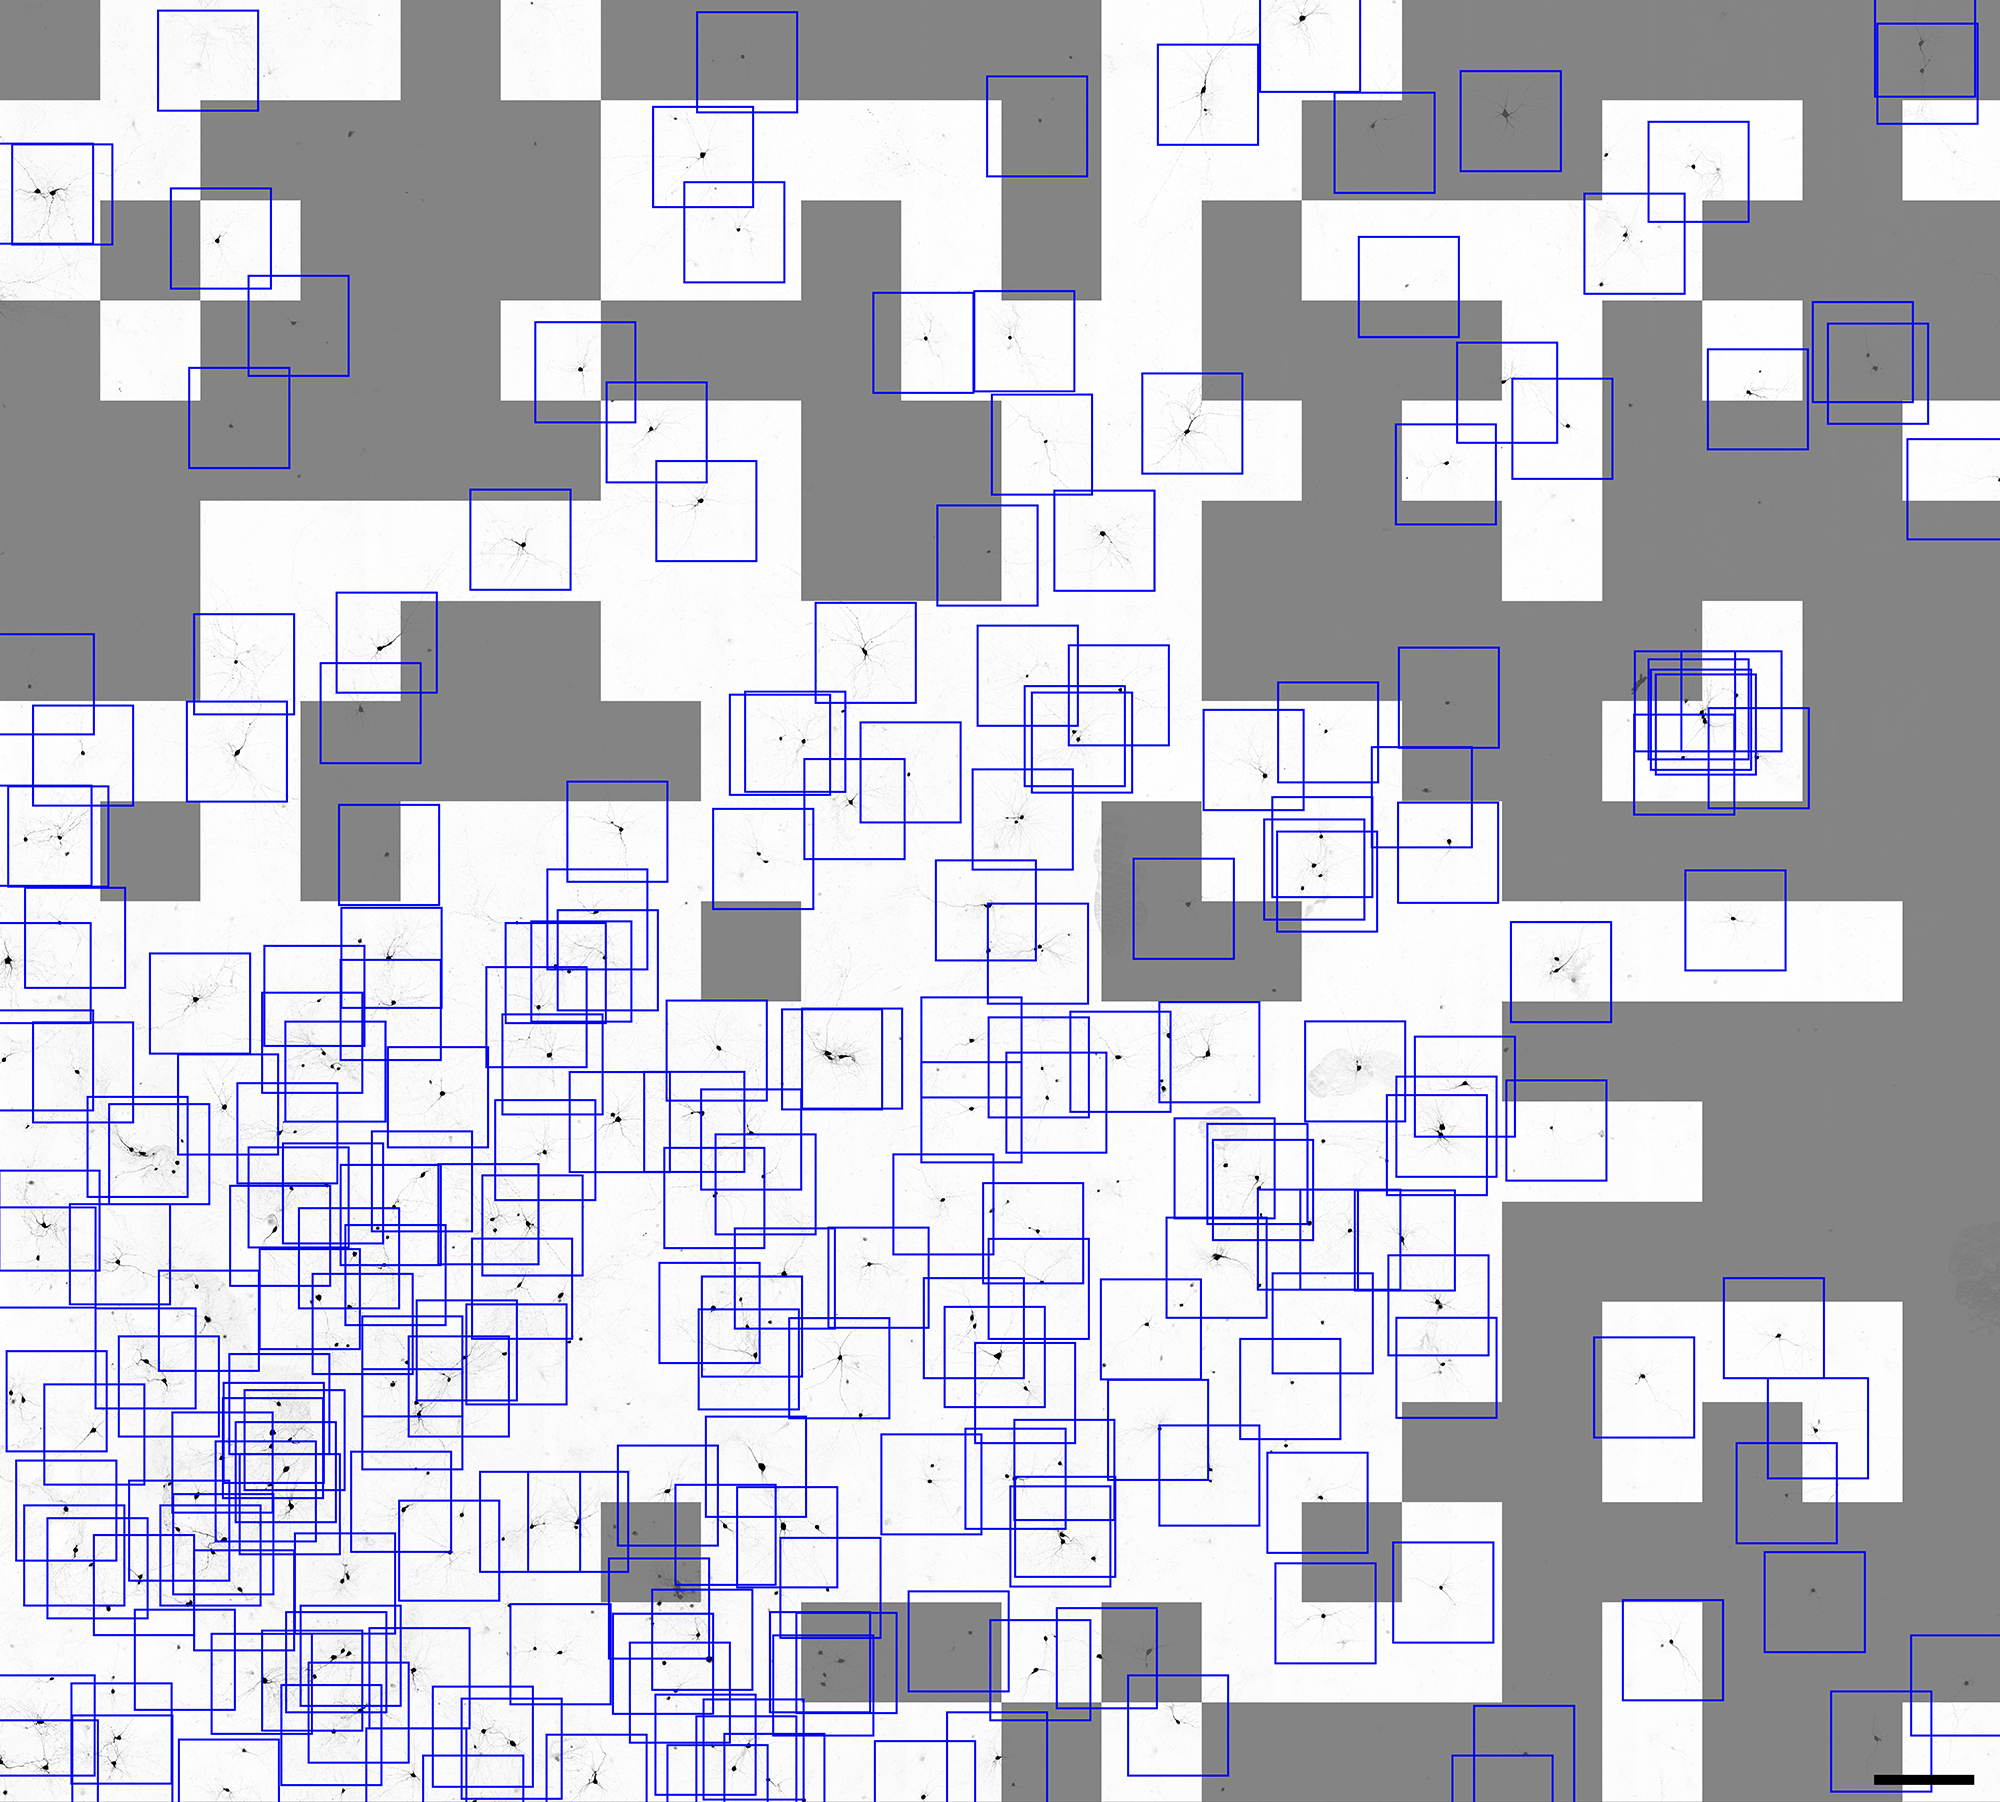
\includegraphics[height=0.50\textwidth]{fig11b}
	\end{tabular}
	\caption{Example of neuron detection in high-content fluorescence microscopy images. The images are shown with inverted intensities (dark grayscale parts) compared to the original. Left: One of the eight images used in the cross-validation experiment. Right: A new image acquired in a later experiment and not used in the cross-validation experiment. This detection example uses the SVM classifier with the SIFT230 feature set to classify square patches from a superimposed grid as neuron (bright grayscale) versus non-neuron (dark grayscale). The detected neuron regions correspond very well with the expert human annotations (blue squares). Scale bars: 500 $\mu$m.}
	\label{ch5_fig11}
\end{figure}
In the spirit of Occam's razor principle \cite{iacca2012ockham, hong2013particle, ebrahimpour2017occam}, which considers the simplest explanation of natural phenomena to be the closest to the truth, additional experimentation sought for the smallest possible classification model capable of determining with high accuracy whether or not a new unseen image patch contains neuron structures. Generally speaking, in order to achieve good generalization in a classification task, it is required to have a sufficient number of samples and to minimize model complexity \cite{gupta2017sparse}. Since the data used in this study is currently rather limited, the investigation was initiated by considering state-of-the-art classification algorithms involving explicit calculation of features, and using state-of-the-art algorithms for extracting a very wide variety and large number of features. In the future, when more annotated data becomes available for this study, deep learning approaches are expected to be good and possibly superior alternatives, as they have been very successful in many other applications \cite{lecun2015deep, bianchini2014complexity, greenspan2016guest, tajbakhsh2016convolutional, shaikhina2017handling, litjens2017survey, shen2017deep}. To get an impression of their performance on current data, a pilot experiment was performed with three convolutional neural networks (\gls{cnn}s). The first was a home-built network (HBN17) with 17 convolutional layers, interspersed with six max-pooling layers, and followed by two fully connected layers outputting the two class probabilities (neuron versus background). The second network was VGG19 \cite{simonyan2014very}, with incorporated modification due to the image patch sizes. Namely, in the presented study, patch sizes are more than four times larger than what VGG19 was originally designed for. This increases the number of network parameters and thus the memory usage to the point that the ability to train the network on our available computers was severely limited. Therefore the number of filters was reduced in the convolution layers by a factor of 16. Also, the network returns only two class probabilities to match this application. The third network was ResNet50 \cite{he2016deep} modified so as to return only two class probabilities. Categorical cross-entropy \cite{ghosh2017robust} was used as the loss function when training the networks, and Adam \cite{kingma2014adam} as the optimizer. The networks were trained on the same balanced data set as the classifiers studied in this work and were tested using the same 3 $\times$ 10-fold cross-validation approach. The results showed that VGG19 performed best (median AUROC of 0.960), followed by ResNet50 (median AUROC of 0.947), and HBN17 (median AUROC of 0.936). Clearly the networks are as yet outperformed by the best classifiers considered in this study. Better results may be achieved not only by acquiring more data but also by applying stronger data augmentation than done here. Another potential direction for future research would be to reformulate the problem as a multiclass detection challenge, distinguishing not only between neurons and background, but also incomplete or out-of-focus neurons, astrocytes, and artifacts.

Achieving AUROC values between 0.97 and 0.98, the best models considered in the present study are already very suitable for detecting neurons in high-content fluorescence microscopy images. As an example the model using the SVM classifier and the SIFT230 feature set was applied to one of the dataset images (Fig.~\ref{ch5_fig11}). In addition, to investigate the generalizability, it was also applied to a new, ``unseen'' image from a new experiment. In that experiment, to introduce some variability, a transfection method with higher efficiency \cite{bredenbeek1993sindbis} was used, resulting in higher intensities and larger numbers of neurons in the field of view. In both images, to detect the neurons, a very simple and low-cost detection approach was used, where square patches (same patch size as used throughout this study) from a superimposed grid were classified individually as neuron versus non-neuron. If needed, more sophisticated (but more computationally costly) detection schemes with higher localization precision could be easily made, by using finer grids with overlapping patches (keeping the same patch size) and segmenting the positive responses. In high-content fluorescence microscopy neuron image analysis, detection is only the first step in a much more comprehensive pipeline developed for fully automated neuron screening, where the actual neuron reconstruction and downstream morphological analysis is based on much higher-resolution images taken at the locations detected in the low-resolution high-content images. The results presented in this study indicate that machine learning approaches are very suitable for the initial detection task and can drastically reduce the high-resolution scan time and analysis.